%
% Template for DAS course projects
%
\documentclass[a4paper,11pt,oneside]{book}
\usepackage[latin1]{inputenc}
\usepackage[english]{babel}
\usepackage{amsfonts}
\usepackage{amsmath}
\usepackage{bm}
\usepackage{amssymb,amsmath,color}
\usepackage{cite}
\usepackage{graphicx}
\usepackage{float}
\usepackage{caption}
\usepackage{subcaption}
\usepackage[hidelinks]{hyperref}
\usepackage{cleveref}
\usepackage{booktabs}
\usepackage[inline]{enumitem}

\begin{document}
\pagestyle{myheadings}

\def\N{{\mathbb{N}}}
\def\R{{\mathbb{R}}}
\def\z{{\bm{z}}}
\def\Q{{\bm{Q}}}
\def\r{{\bm{r}}}
\def\p{{\bm{p}}}


%%%%%%%%%%% Cover %%%%%%%%%%%
\thispagestyle{empty}                                                 
\begin{center}                                                            
    \vspace{5mm}
    {\LARGE UNIVERSIT\`A DI BOLOGNA} \\                       
      \vspace{5mm}
\end{center}
\begin{center}
  
\includegraphics[scale=.27]{figs/logo_unibo}
\end{center}
\begin{center}
      \vspace{5mm}
      {\LARGE School of Engineering} \\
        \vspace{3mm}
      {\Large Master Degree in Artificial Intelligence} \\
      \vspace{20mm}
      {\LARGE Distributed Autonomous Systems} \\
      \vspace{5mm}{\Large\textbf{Multi-Robot Distributed Optimization}}                  
      \vspace{15mm}
\end{center}
\begin{minipage}{0.48\linewidth}
      \raggedright
     {\large Professors:}\\
     \textbf{Giuseppe Notarstefano} \\
     \textbf{Ivano Notarnicola} \\        
%      \vspace{13mm}
\end{minipage}
\begin{minipage}{0.48\linewidth}
      \raggedleft
      {\large Students:}\\
      \textbf{\@ Valerio Costa} \\
      \textbf{\@ Tian Cheng Xia} \\  
\end{minipage}
\begin{center}
\vfill
      {\large Academic year \@2024/2025} \\
\end{center}



\newpage
\thispagestyle{empty}

%%%%%%%%%%% Abstract %%%%%%%%%%%%
\begin{center}
\chapter*{}
\thispagestyle{empty}
{\Huge \textbf{Abstract}}\\
\vspace{15mm}
\end{center}

Multi-robot target localization and multi-robot positioning are two tasks that can be tackled in a distributed fashion. In this project, we solve both of them and experiment with their capabilities: the former is implemented in Python while the latter both in Python and ROS2. The first task can be solved using the gradient tracking algorithm, while the second one as an aggregative optimization problem. For the tracking task, our experimental results show that communication graph connectivity and number of agents have significant effects in convergence speed and accuracy. For the aggregative task, we observed that all graph patterns behave similarly, independently of the number of robots. Moreover, experiments with different loss hyperparameters show that the constraints defined in the loss function can be easily tuned and the movement of the robots is coherent with the assigned weights.

\tableofcontents \thispagestyle{empty}
% \listoffigures\thispagestyle{empty}

%%%%%%%%%% Introduction %%%%%%%%%%
\chapter*{Introduction}
\addcontentsline{toc}{chapter}{Introduction}

\section*{Motivations} 

The project aims at implementing distributed algorithms to solve two specific tasks. The first one, which can be solved using the gradient tracking algorithm, involves the problem of distributed target localization where some tracking robots want to reach consensus in estimating the position of some targets for which only noisy measurements are known. The second one, which is an aggregative optimization problem, consists of positioning robots balancing the requirements of being close to private targets and keeping the whole fleet tight. For both tasks, we experiment with the implementation to assess their results in terms of correctness, convergence, and scalability.

The rest of the report is structured as follows: in \Cref{ch:quadratic}, we implement the gradient tracking algorithm for quadratic functions. In \Cref{ch:localization}, we solve and show the results for the task of target localization. In \Cref{ch:aggregative}, we present the solution and the experiments for the task of robots positioning.


\section*{Contributions}

This project provides a small comparison benchmark of some distributed algorithms. These results, although limited, show the effectiveness of these algorithms in solving some tasks for which taking a centralized approach is not realistic. 

In practical terms, most of the work has been done in pair programming and both group members have contributed equally to the implementation.




\setcounter{page}{1}
\chapter{Gradient Tracking with Quadratic Functions} \label{ch:quadratic}



\section{Problem definition}

The first part of the first task consists of implementing the gradient tracking algorithm generalized in $\R^d$ and experimenting with the implementation using quadratic functions, which we define in the usual way as:
\[
      f(\z) = \frac{1}{2} \z^T \Q \z + \r^T \z
      \quad
      \nabla f(\z) = \Q \z + \r,
\]
where $\z \in \R^{d}$ are the parameters, and $\Q \in \R^{d \times d}$ (positive definite) and $\r \in \R^{d}$ are the coefficients of the function. More in details, given $N \in \N$ agents where each has associated a private quadratic function $f_i$ with its own coefficients $\Q_i$ and $\r_i$, the goal is to use the gradient tracking algorithm to solve the following problem:
\[
      \min_{\z} \sum_{i=1}^{N} f_i(\z),
\]
where $\z \in \R^{d}$ are the decision variables. In other words, the global cost function is the summation of all private quadratic functions and all agents should reach a consensus point that minimizes it.

\section{Code structure} \label{sec:code_quadratic}
The code provided is structured with the following modules:
\begin{description}
      \item[\texttt{algorithm.py}] contains the functions to run the distributed gradient tracking algorithm and the centralized gradient descent.
      \item[\texttt{loss.py}] defines the quadratic function implemented as a Python class.
      \item[\texttt{plot.py}] provides all the functions used to plot the cost, the gradient norm, and the distance to the optimum.
      \item[\texttt{scenarios.py}] with the functions to create the communication graph and to initialize the problem of minimizing quadratic functions.
      \item[\texttt{utils.py}] implements the utility metric to compute the average consensus error.
\end{description}
In practice, all experiments can be executed from the \texttt{main\_quadratic.py} script.



\section{Experiments}

We analyze the behavior with quadratic functions through the definition of different scenarios with different kinds of graph patterns (in particular: complete, binomial with edge probability of $0.3$, cycle, star, and path graph). The configurations we test are the following:
\begin{itemize}
      \item A small problem ($5$ agents in $\R^3$),
      \item A problem with higher dimensionality ($5$ agents in $\R^{15}$),
      \item A problem with many agents ($15$ and $30$ agents in $\R^3$),
      \item A problem with many agents in higher dimensionality ($15$ and $30$ agents in $\R^{15}$).
\end{itemize}
In addition, we perform a comparison between the distributed gradient tracking algorithm and the centralized one. 

For compactness in the discussion, in the rest of this report we show the results with a single initialization seed and, if not specified, it indicates that the results are consistent across different initializations. Also, for readability, for quadratic functions we report the distance to the optimum in semi-logarithmic scale instead of the cost itself which can be negative.


\subsection{Comparison between different graph patterns}

\begin{figure}[h!]
      \centering
      \begin{subfigure}[h]{0.43\linewidth}
            \centering
            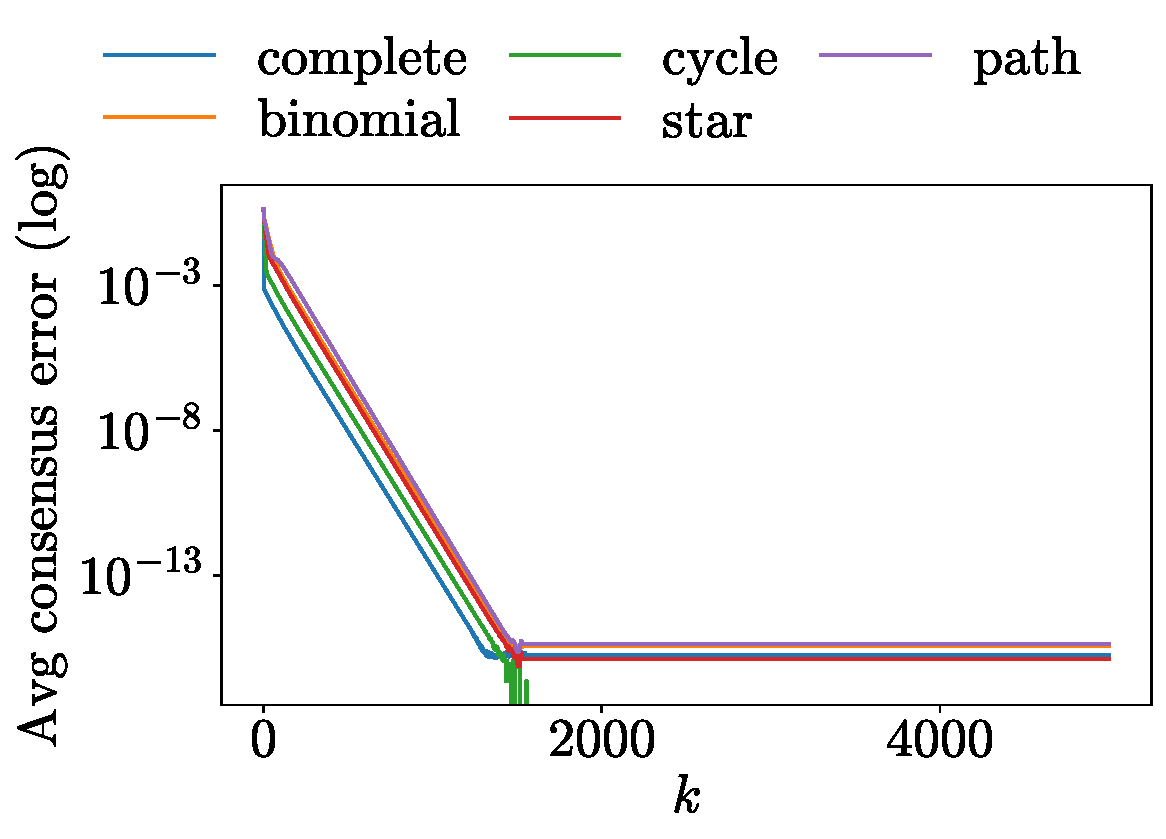
\includegraphics[width=\linewidth]{./figs/quadratic/5_3/consensus.pdf} 
            \caption{$5$ agents in $\R^{3}$}
      \end{subfigure}
      \hfill
      \begin{subfigure}[h]{0.43\linewidth}
            \centering
            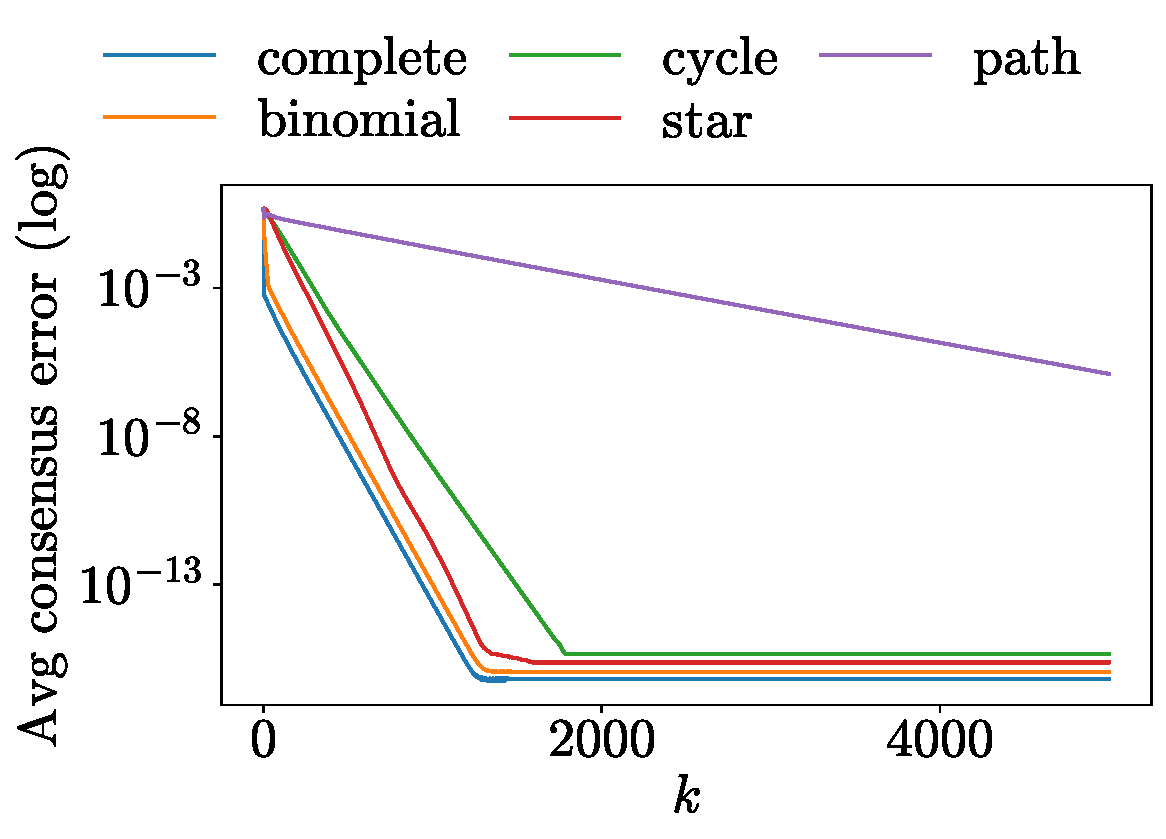
\includegraphics[width=\linewidth]{./figs/quadratic/15_3/consensus.pdf} 
            \caption{$15$ agents in $\R^{3}$}
      \end{subfigure}
      \caption{Consensus error for quadratic function minimization}
      \label{fig:quadratic_consensus}
\end{figure}

We start the analysis by first inspecting the consensus error of the algorithm. In \Cref{fig:quadratic_consensus}, we report the average consensus error in the cases of $5$ and $15$ agents. The general behavior that can be observed is that in all cases consensus is reached, in line with the theoretical guarantees of the algorithm. However, it can also be seen that consensus is reached faster when the communication graph has more connectivity, indicating that, as intuition would suggest, being able to communicate with more agents helps on this aspect. Also, although not reported for compactness, these observations hold for the other scenarios as well.


\begin{figure}[h!]
      \centering
      \begin{subfigure}[h]{0.42\linewidth}
            \centering
            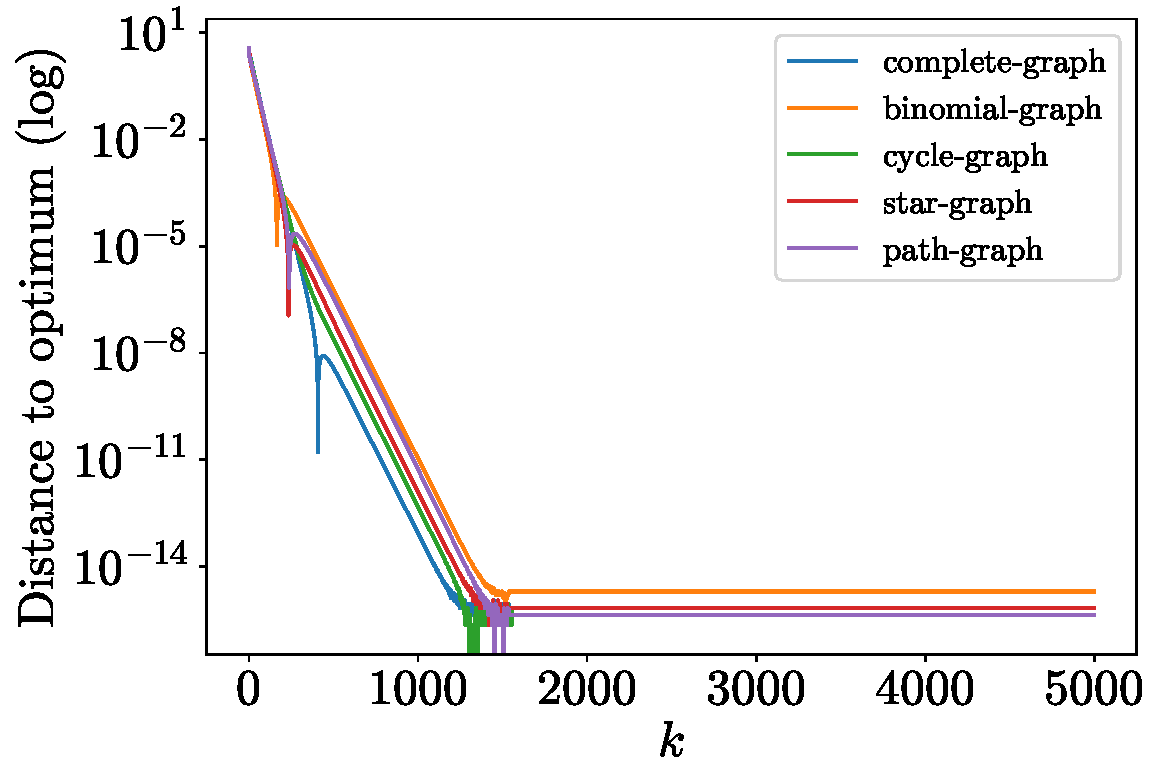
\includegraphics[width=\linewidth]{./figs/quadratic/5_3/distance.pdf} 
            \caption{Distance to optimum}
      \end{subfigure}
      \hfill
      \begin{subfigure}[h]{0.42\linewidth}
            \centering
            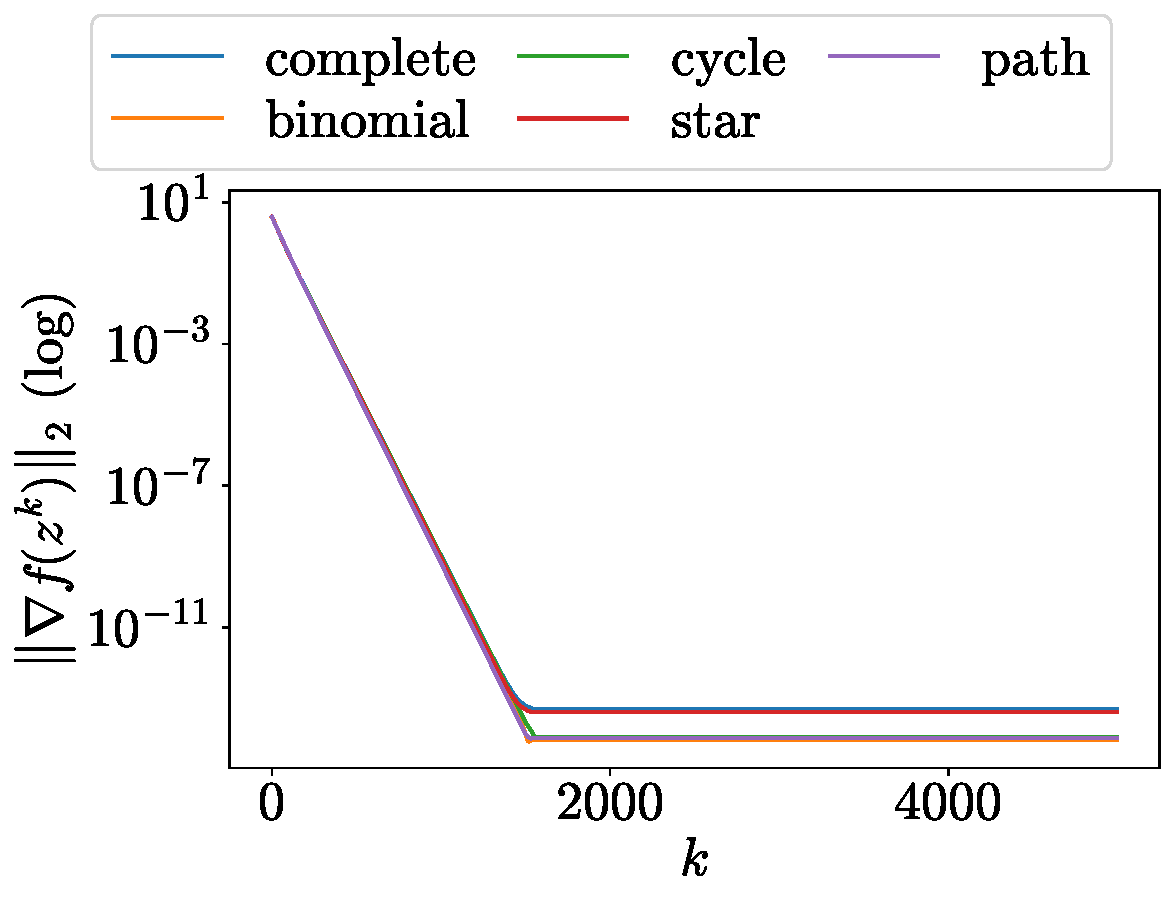
\includegraphics[width=\linewidth]{./figs/quadratic/5_3/gradient.pdf} 
            \caption{Gradient norm evolution}
      \end{subfigure}
      \caption{Quadratic function minimization with $5$ agents in $\R^{3}$}
      \label{fig:quadratic_5_3}
\end{figure}

\begin{figure}[h!]
      \centering
      \begin{subfigure}[h]{0.42\linewidth}
            \centering
            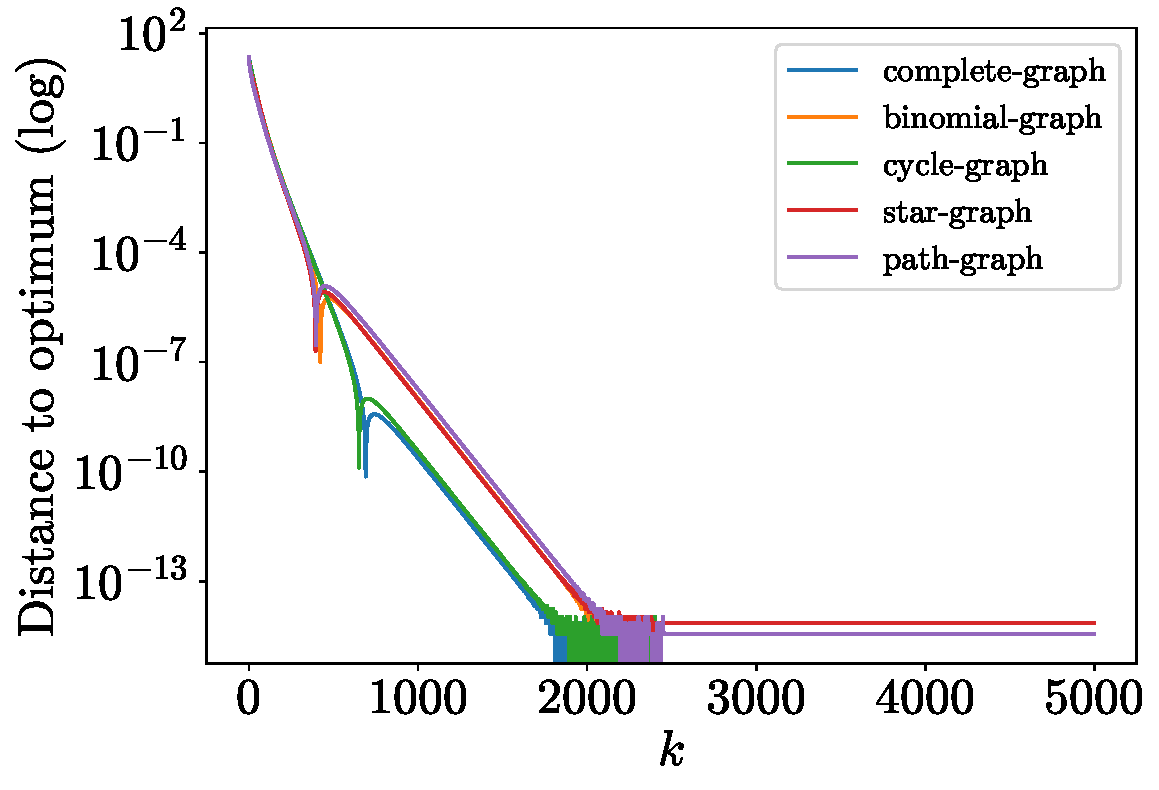
\includegraphics[width=\linewidth]{./figs/quadratic/5_15/distance.pdf} 
            \caption{Distance to optimum}
      \end{subfigure}
      \hfill
      \begin{subfigure}[h]{0.42\linewidth}
            \centering
            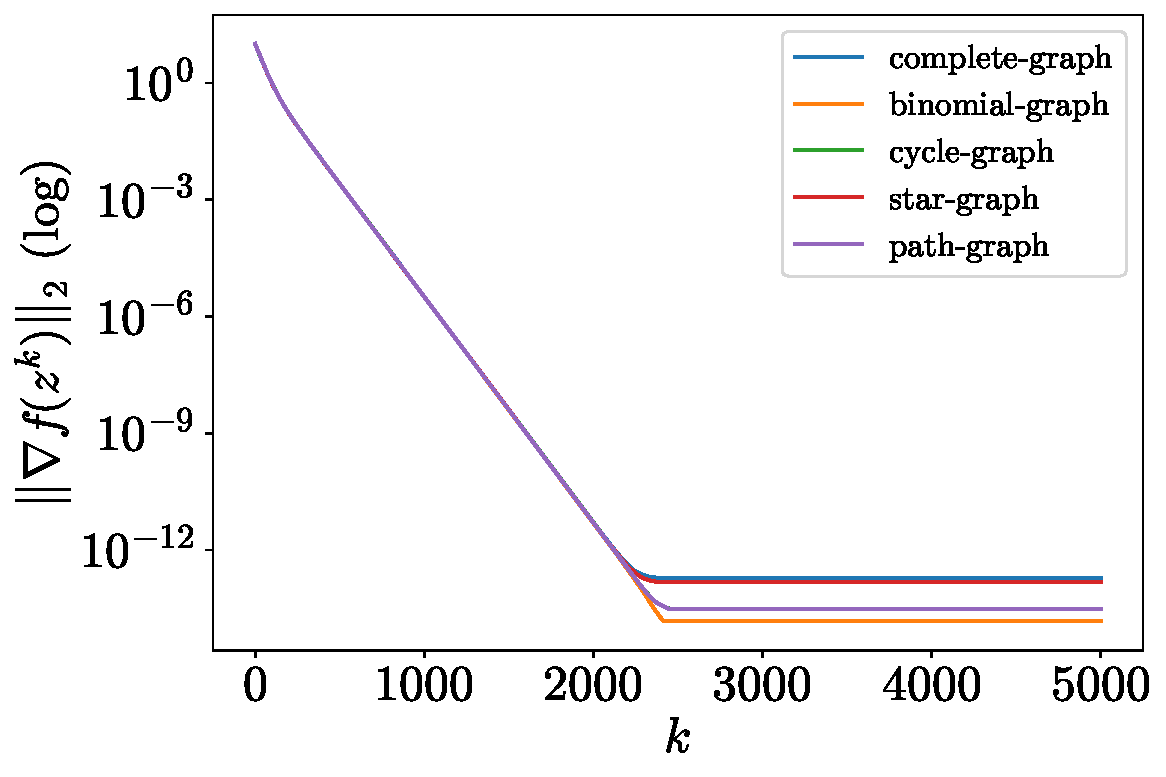
\includegraphics[width=\linewidth]{./figs/quadratic/5_15/gradient.pdf} 
            \caption{Gradient norm evolution}
      \end{subfigure}
      \caption{Quadratic function minimization with $5$ agents in $\R^{15}$}
      \label{fig:quadratic_5_15}
\end{figure}

In terms of cost function instead, for the small problem we can observe from \Cref{fig:quadratic_5_3} a relatively smooth improvement of the cost function and an exponentially decreasing gradient in all cases, as expected from theoretical results. By experimenting with variables of higher dimensionality, we can observe from \Cref{fig:quadratic_5_15} that the behavior of both the cost and its gradient are very similar to the previous case with the only difference that more iterations are required to reach full convergence, indicating that dimensionality is marginal in changing the difficulty of the problem. 


\begin{figure}[t!]
      \centering
      \begin{subfigure}[h]{0.42\linewidth}
            \centering
            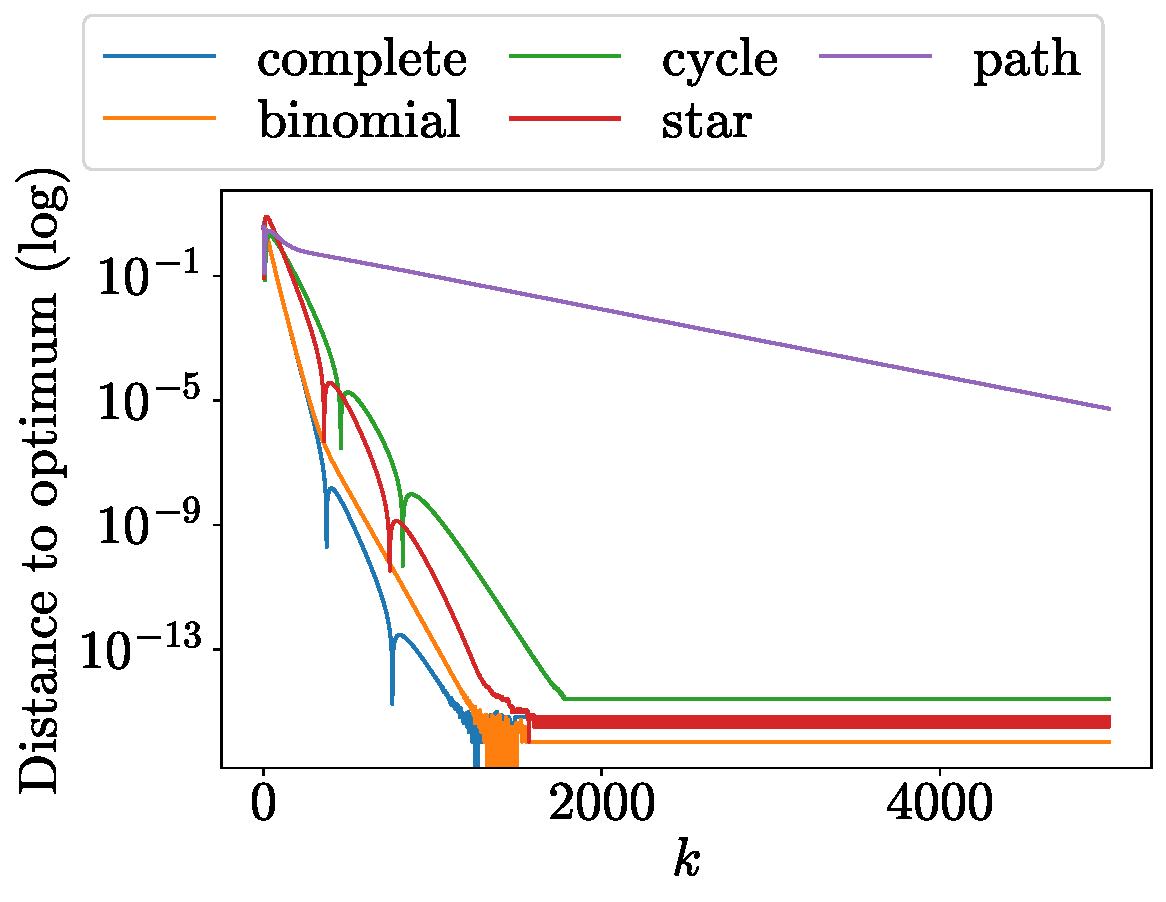
\includegraphics[width=\linewidth]{./figs/quadratic/15_3/distance.pdf} 
            \caption{Distance to optimum}
      \end{subfigure}
      \hfill
      \begin{subfigure}[h]{0.42\linewidth}
            \centering
            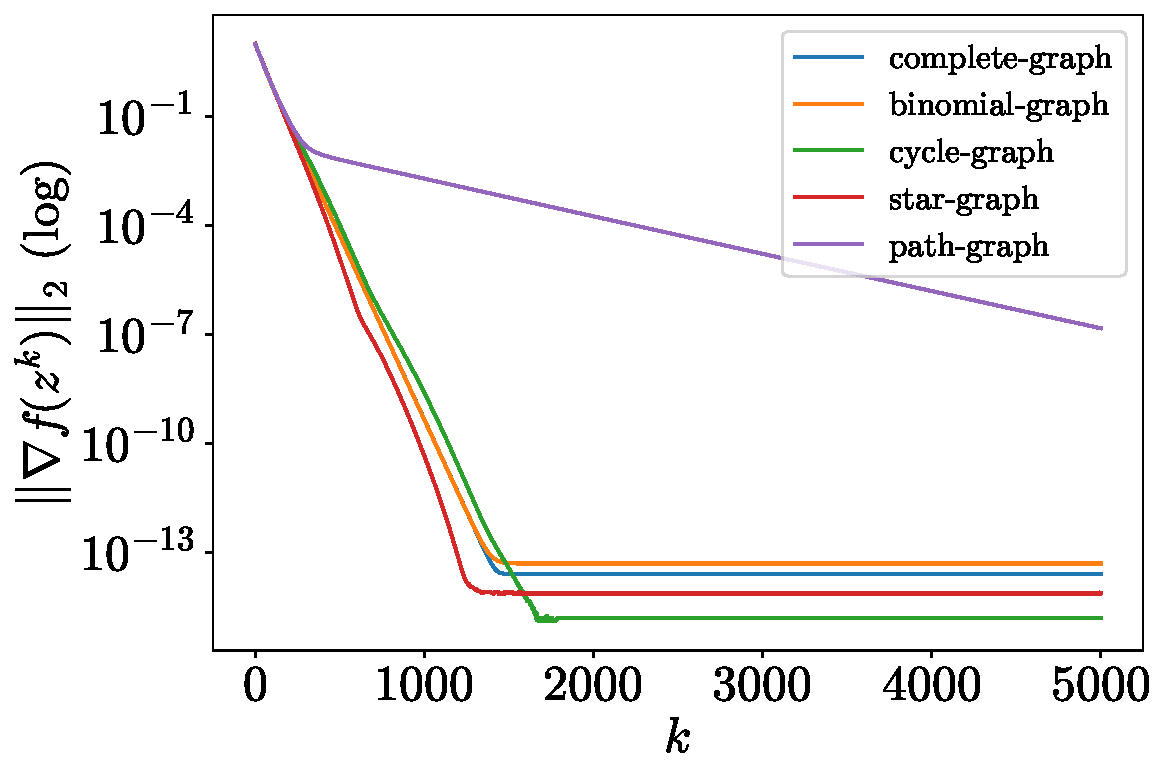
\includegraphics[width=\linewidth]{./figs/quadratic/15_3/gradient.pdf} 
            \caption{Gradient norm evolution}
      \end{subfigure}
      \caption{Quadratic function minimization with $15$ agents in $\R^{3}$}
      \label{fig:quadratic_15_3}
\end{figure}

\begin{figure}[t!]
      \centering
      \begin{subfigure}[h]{0.42\linewidth}
            \centering
            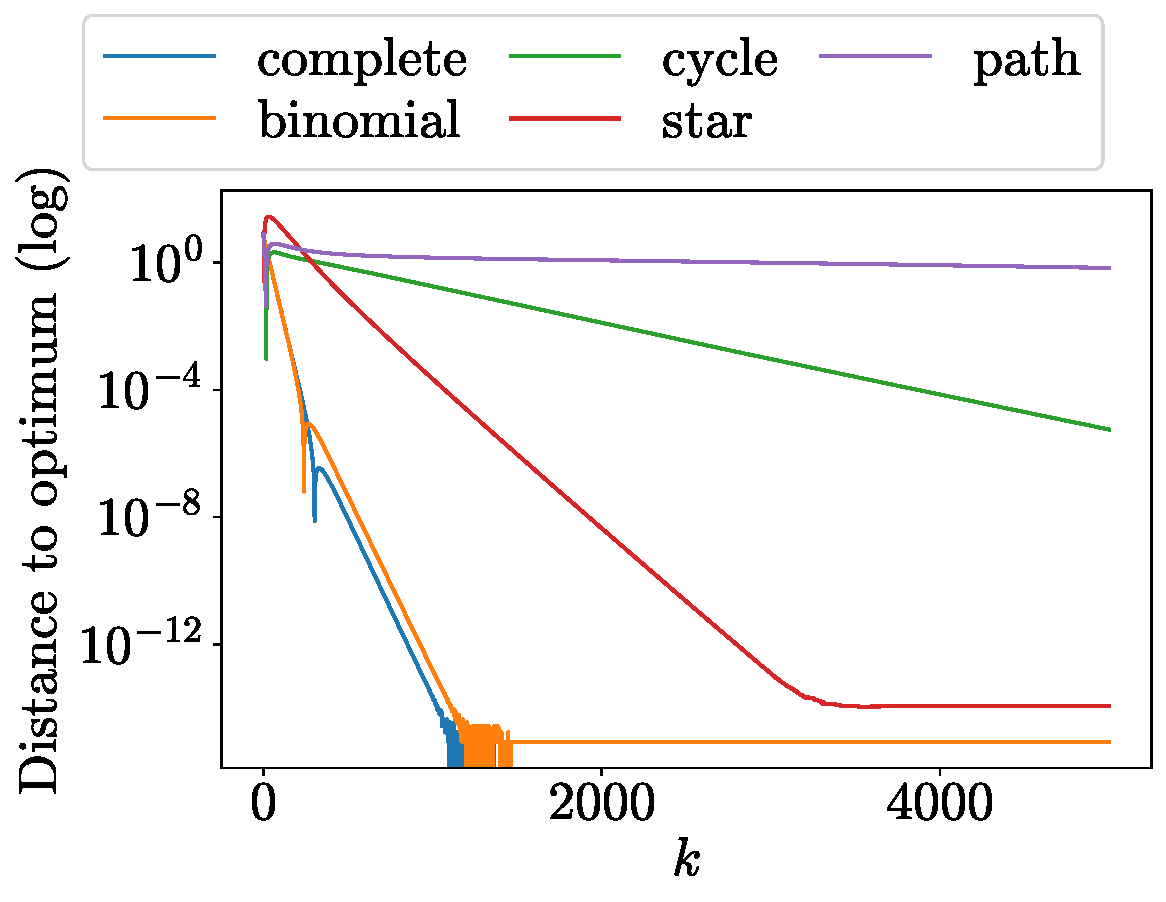
\includegraphics[width=\linewidth]{./figs/quadratic/30_3/distance.pdf} 
            \caption{Distance to optimum}
      \end{subfigure}
      \hfill
      \begin{subfigure}[h]{0.42\linewidth}
            \centering
            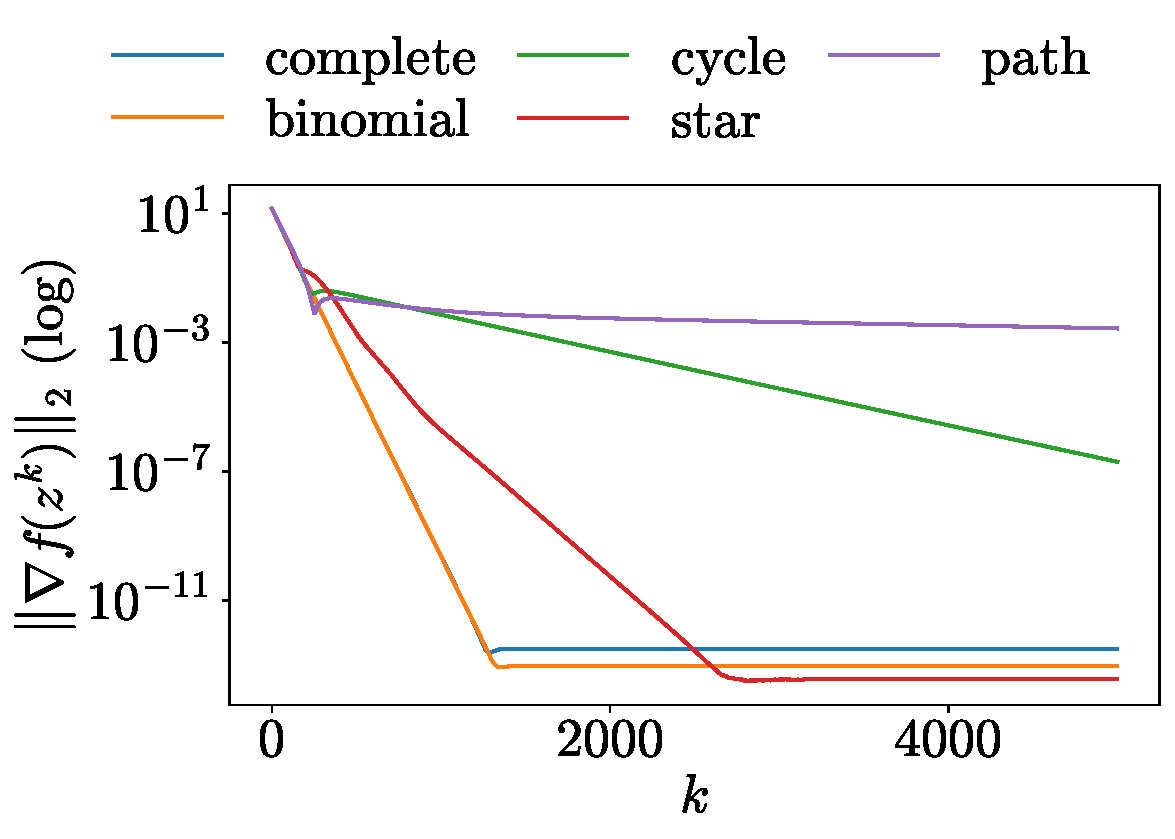
\includegraphics[width=\linewidth]{./figs/quadratic/30_3/gradient.pdf} 
            \caption{Gradient norm evolution}
      \end{subfigure}
      \caption{Quadratic function minimization with $30$ agents in $\R^{3}$}
      \label{fig:quadratic_30_3}
\end{figure}

In the case of many agents with lower dimensionality, we can observe from \Cref{fig:quadratic_15_3,fig:quadratic_30_3} that the cost function does not reach the optimum within the given number of iterations with the configurations using poorly connected communication graphs, indicating again that connectivity is important with higher numbers of agents. This can be explained by the fact that, by adding more agents, the overall problem includes more local losses and becomes more difficult to solve in a distributed way. Lastly, by increasing variable dimensionality, from \Cref{fig:quadratic_15_15,fig:quadratic_30_15} we can observe the same convergence behavior as in the case of low dimensional variables, confirming that on this aspect the problem is not significantly affected.


\begin{figure}[h!]
      \centering
      \begin{subfigure}[h]{0.42\linewidth}
            \centering
            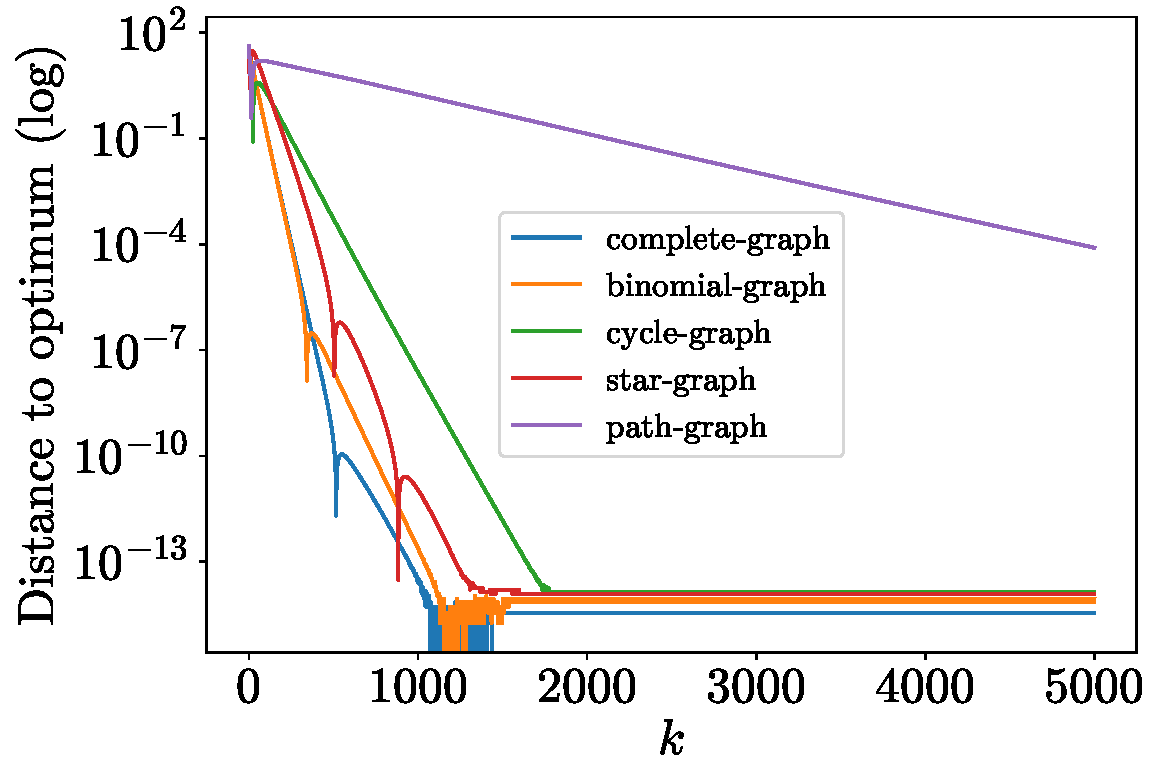
\includegraphics[width=\linewidth]{./figs/quadratic/15_15/distance.pdf} 
            \caption{Distance to optimum}
      \end{subfigure}
      \hfill
      \begin{subfigure}[h]{0.42\linewidth}
            \centering
            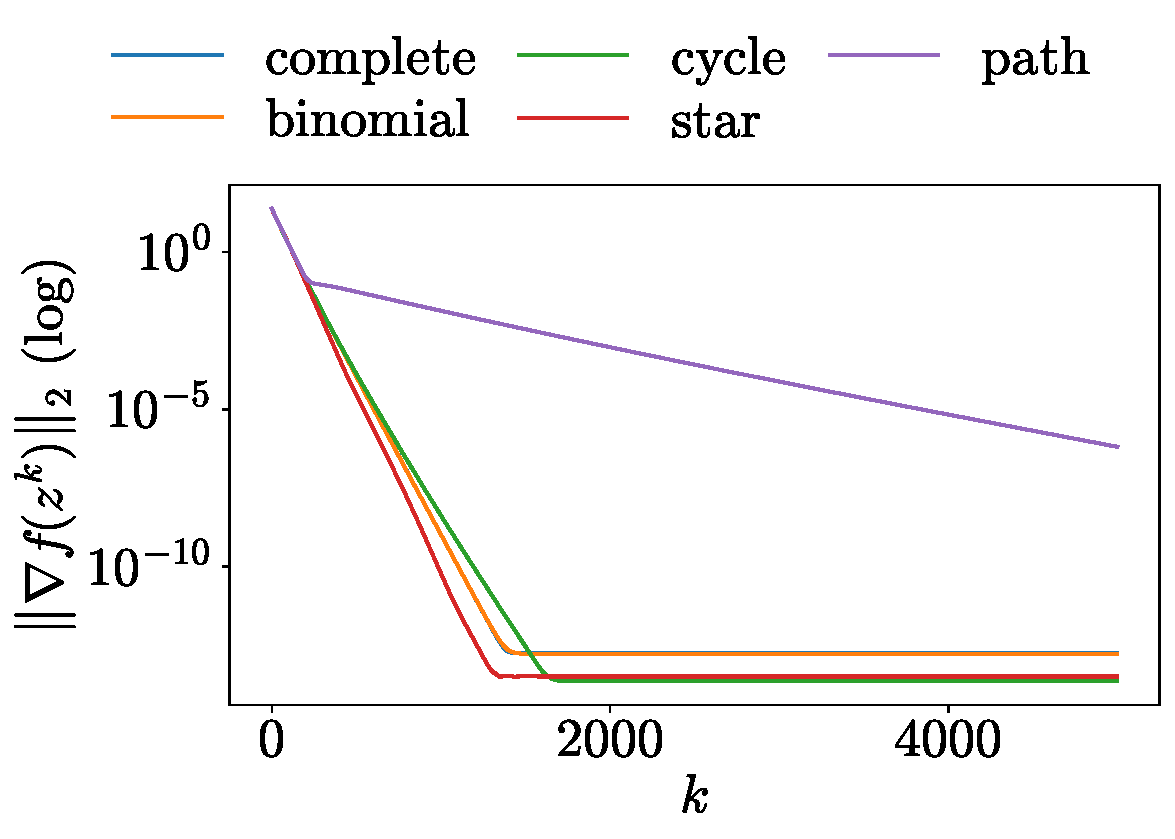
\includegraphics[width=\linewidth]{./figs/quadratic/15_15/gradient.pdf} 
            \caption{Gradient norm evolution}
      \end{subfigure}
      \caption{Quadratic function minimization with $15$ agents in $\R^{15}$}
      \label{fig:quadratic_15_15}
\end{figure}

\begin{figure}[h!]
      \centering
      \begin{subfigure}[h]{0.42\linewidth}
            \centering
            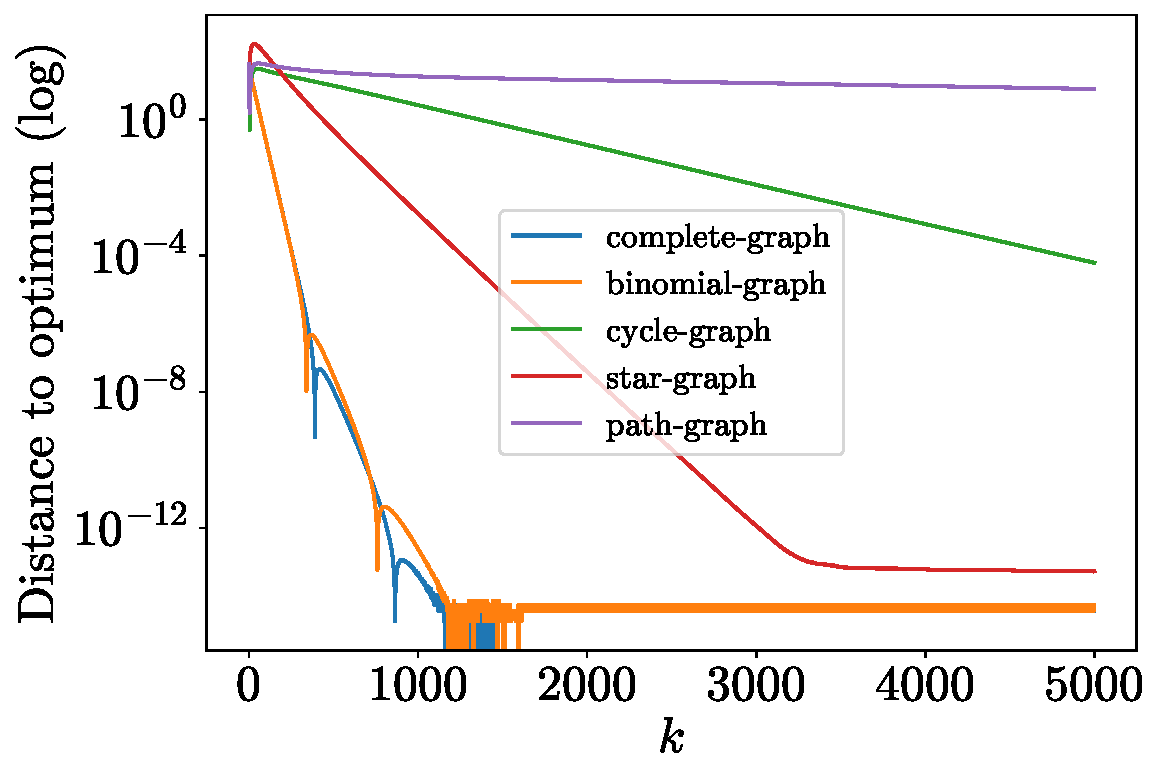
\includegraphics[width=\linewidth]{./figs/quadratic/30_15/distance.pdf} 
            \caption{Distance to optimum}
      \end{subfigure}
      \hfill
      \begin{subfigure}[h]{0.42\linewidth}
            \centering
            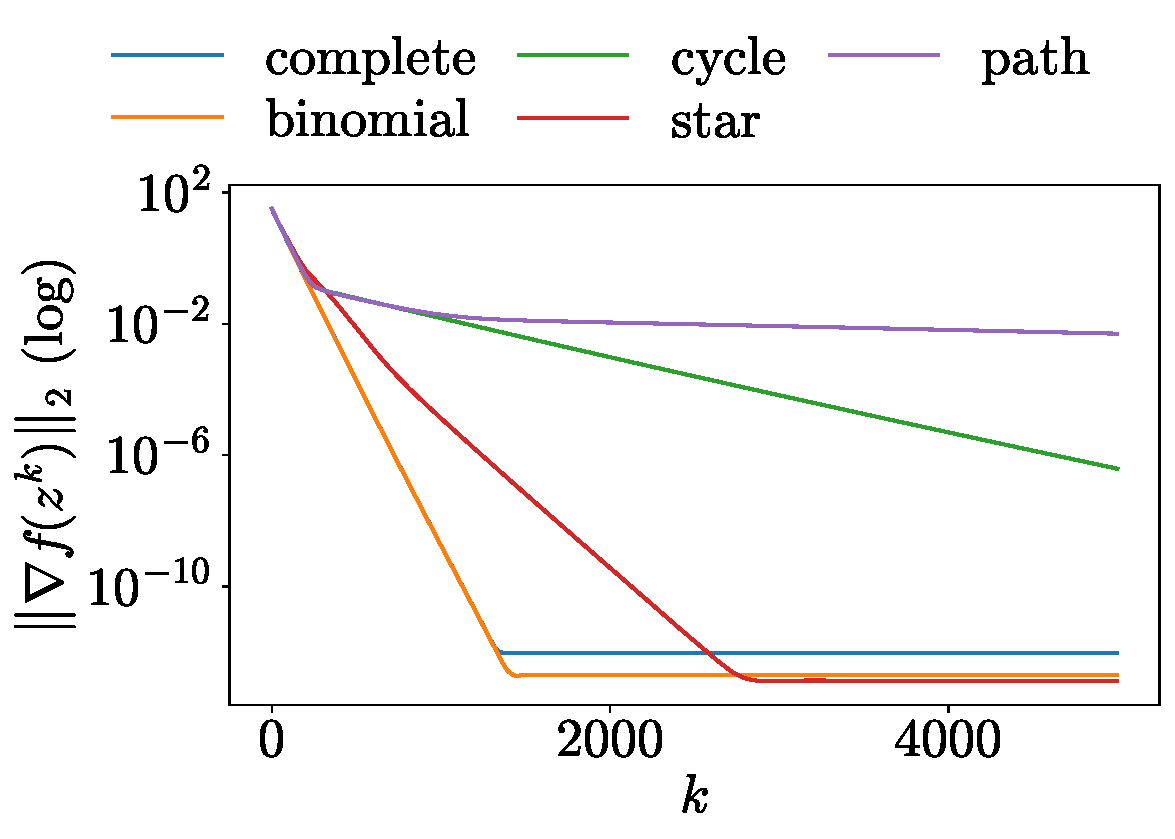
\includegraphics[width=\linewidth]{./figs/quadratic/30_15/gradient.pdf} 
            \caption{Gradient norm evolution}
      \end{subfigure}
      \caption{Quadratic function minimization with $30$ agents in $\R^{15}$}
      \label{fig:quadratic_30_15}
\end{figure}



\subsection{Comparison with centralized gradient}

Following the previous results, we select the best performing configuration and compare it with the centralized gradient method. In \Cref{fig:quadratic_centralized_15_3} we can observe the results with $15$ agents and a complete communication graph, but the overall behavior is the same for all configurations. It can be seen that, as one could expect, the centralized gradient method is faster to converge and it is slightly more precise compared to a distributed algorithm as it has available all the global information without relying on estimates obtained from neighbors and therefore it accumulates less numerical errors.

\begin{figure}[t!]
      \centering
      \begin{subfigure}[h]{0.43\linewidth}
            \centering
            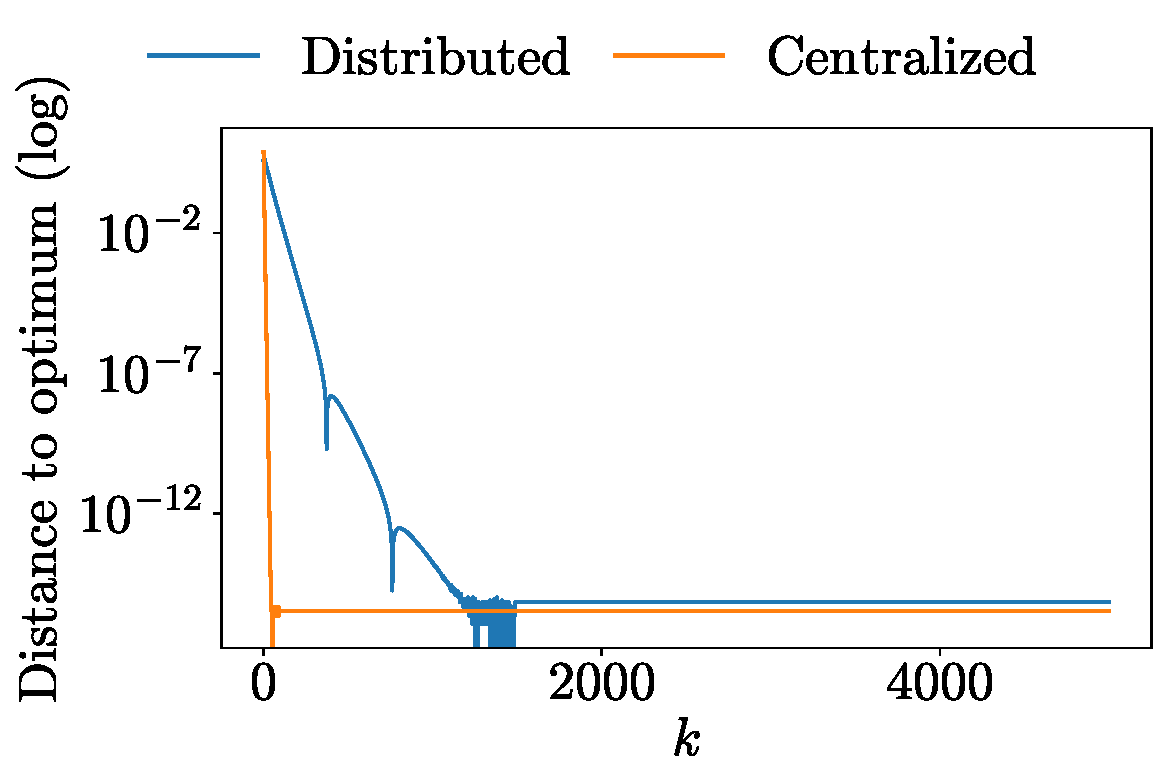
\includegraphics[width=\linewidth]{./figs/quadratic/centralized/distance.pdf} 
            \caption{Distance to optimum}
      \end{subfigure}
      \hfill
      \begin{subfigure}[h]{0.43\linewidth}
            \centering
            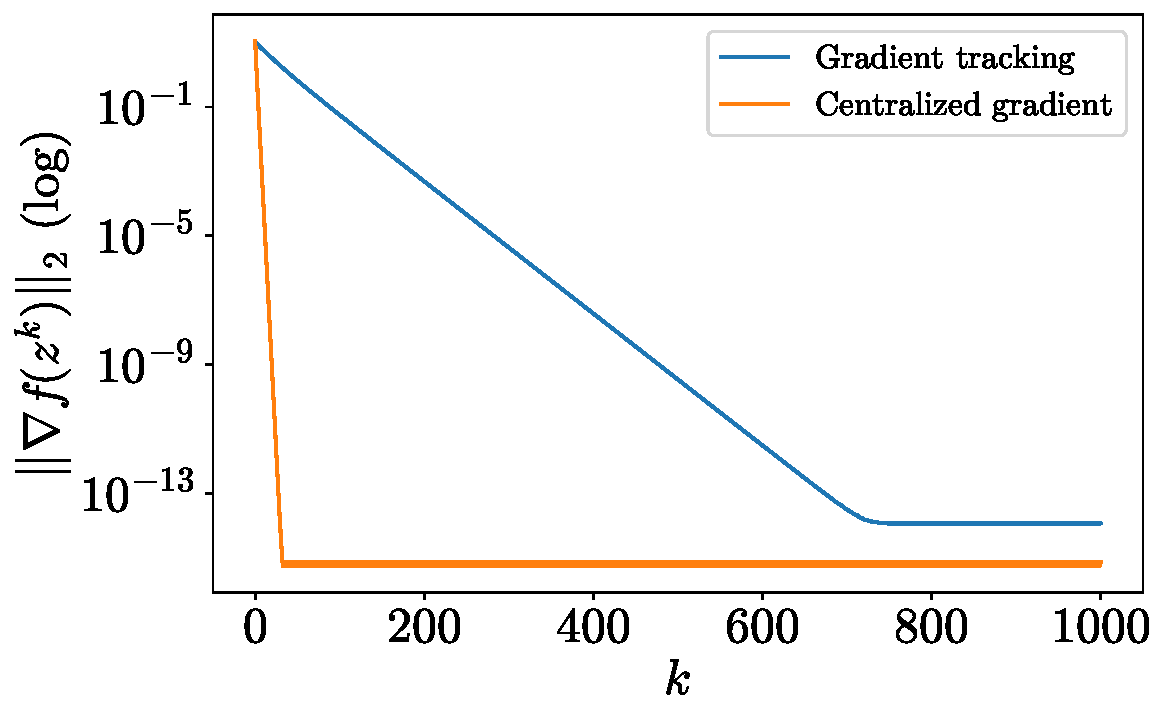
\includegraphics[width=\linewidth]{./figs/quadratic/centralized/gradient.pdf} 
            \caption{Gradient norm evolution}
      \end{subfigure}
      \caption{Quadratic function minimization with $15$ agents in $\R^{3}$ compared to centralized gradient}
      \label{fig:quadratic_centralized_15_3}
\end{figure}




\chapter{Cooperative Multi-Robot Target Localization} \label{ch:localization}


\section{Problem definition}

The problem in the second part of the first task involves a similar context as the previous case. The fundamental difference is that the local losses each agent has to minimize are designed to solve the problem of target localization. More specifically, this problem requires to estimate the position of $N_T \in \N$ fixed targets in a distributed way through $N_R \in \N$ tracking robots. Each robot is located at position $\p_i \in \R^2$ and it is assumed that the distance measured from each robot is noisy. Given the positions $\p_i$ and $\p_\tau$ of the $i$-th robot and the $\tau$-th target, respectively, we model the measured noisy distance $d_{i,\tau}$ from robot $i$ as follows:
\[
      d_{i,\tau} = \Vert \p_i - \p_\tau \Vert + \varepsilon \cdot \texttt{noise},
\]
where $\texttt{noise} \sim P$ is drawn from some distribution $P$ and $\varepsilon \in \R$ is the noise rate that controls how much noise is injected into the measurement.

The local loss each robot $i$ uses is the following:
\[
      \begin{gathered}
            l_i(\z_i) = \sum_{\tau=1}^{N_T} \left( d_{i,\tau}^2 - \Vert \z_{i,\tau} - \p_i \Vert^2 \right)^2
            \quad
            \nabla l_{i}(\z_i) = (\nabla l_{i,1}(\z_{i,1}), \dots, \nabla l_{i,N_T}(\z_{i,N_T}))
            \\
            \nabla l_{i,\tau}(\z_{i,\tau}) = -4 \left( d_{i,\tau}^2 - \Vert \z_{i,\tau} - \p_i \Vert^2 \right) \left( \z_{i,\tau} - \p_i \right),
      \end{gathered}
\]
where $\z_i = (\z_{i,1}, \dots, \z_{i,N_T}) \in \R^{2N_T}$ is the stack of decision variables of robot $i$ containing the estimated positions of the targets $\z_{i,\tau} \in \R^2$ and $\nabla l_i(\z_i) \in \R^{2N_T}$ is the concatenation of the gradients computed with respect to each target.

\section{Code structure}
The code provided is structured with the following modules (considering only the differences from \Cref{sec:code_quadratic}):
\begin{description}
      \item[\texttt{loss.py}] contains the class definition of the target localization loss.
      \item[\texttt{plot.py}] defines all the functions used to plot the loss and the gradient norm.
      \item[\texttt{scenarios.py}] implements the function to initialize the parameters (i.e., the ground truth target positions, initial robot positions, and noisy estimated target distances) and the target localization loss of the problem.
\end{description}
In practice, all the experiments can be executed from the \texttt{main\_tracking.py} script.



\section{Experiments}

We approach the experimentation of this problem by trying different graph patterns and comparing it with the centralized gradient method, similarly to \Cref{ch:quadratic}. At first, we evaluate the performance of the algorithm in the following cases, all with the same type of noise:
\begin{itemize}
      \item A few robots ($5$) with a single target,
      \item A few robots ($5$) with multiple targets ($3$),
      \item Many robots ($15$ and $30$) with multiple targets ($3$).
\end{itemize}

Then, the focus switches to observe how much the performance changes in terms of noise. By fixing the problem configuration, we experiment with varying Gaussian noises, Poisson noises, and noise rates.


\subsection{Comparison between different graph patterns}

In terms of graph patterns, we can observe from \Cref{fig:tracking_5_1,fig:tracking_5_3} that with the same number of robots and increasing number of targets, the number of iterations required to converge is roughly the same. This makes sense as each target is independent to the others and can be tracked in parallel.

\begin{figure}[h!]
      \centering
      \begin{subfigure}[h]{0.4\linewidth}
            \centering
            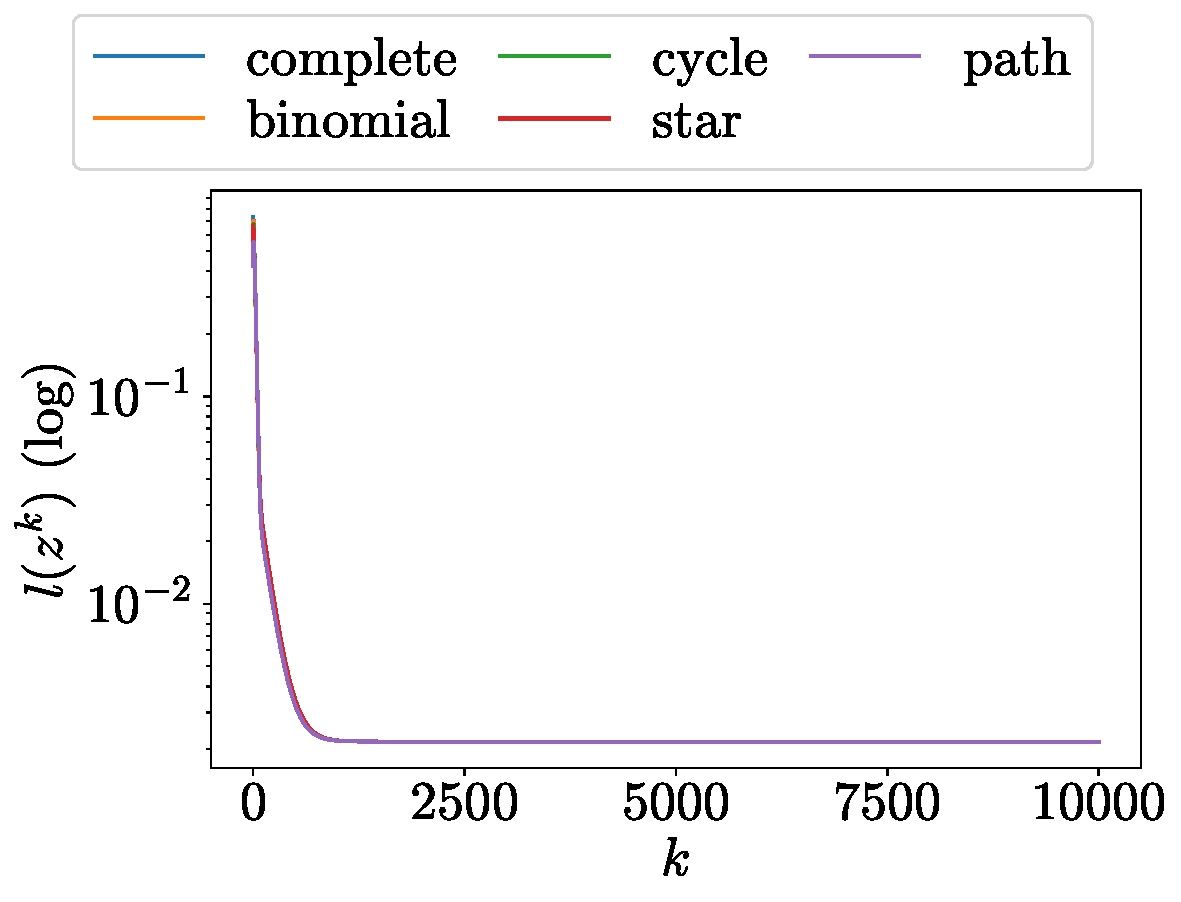
\includegraphics[width=\linewidth]{./figs/tracking/5_1_2/loss.pdf} 
            \caption{Loss evolution}
      \end{subfigure}
      \hfill
      \begin{subfigure}[h]{0.4\linewidth}
            \centering
            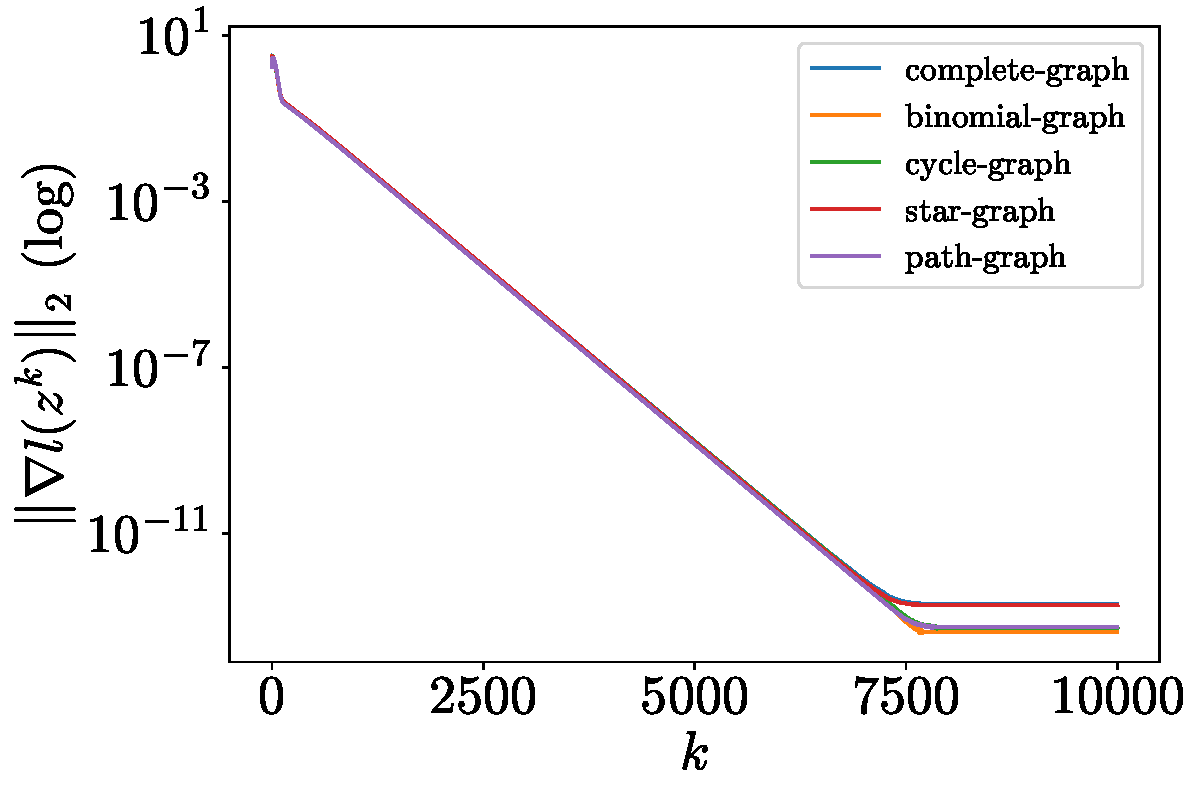
\includegraphics[width=\linewidth]{./figs/tracking/5_1_2/gradient.pdf} 
            \caption{Gradient norm evolution}
      \end{subfigure}
      \caption{Tracking with $5$ robots and $1$ target}
      \label{fig:tracking_5_1}
\end{figure}

\begin{figure}[h!]
      \centering
      \begin{subfigure}[h]{0.4\linewidth}
            \centering
            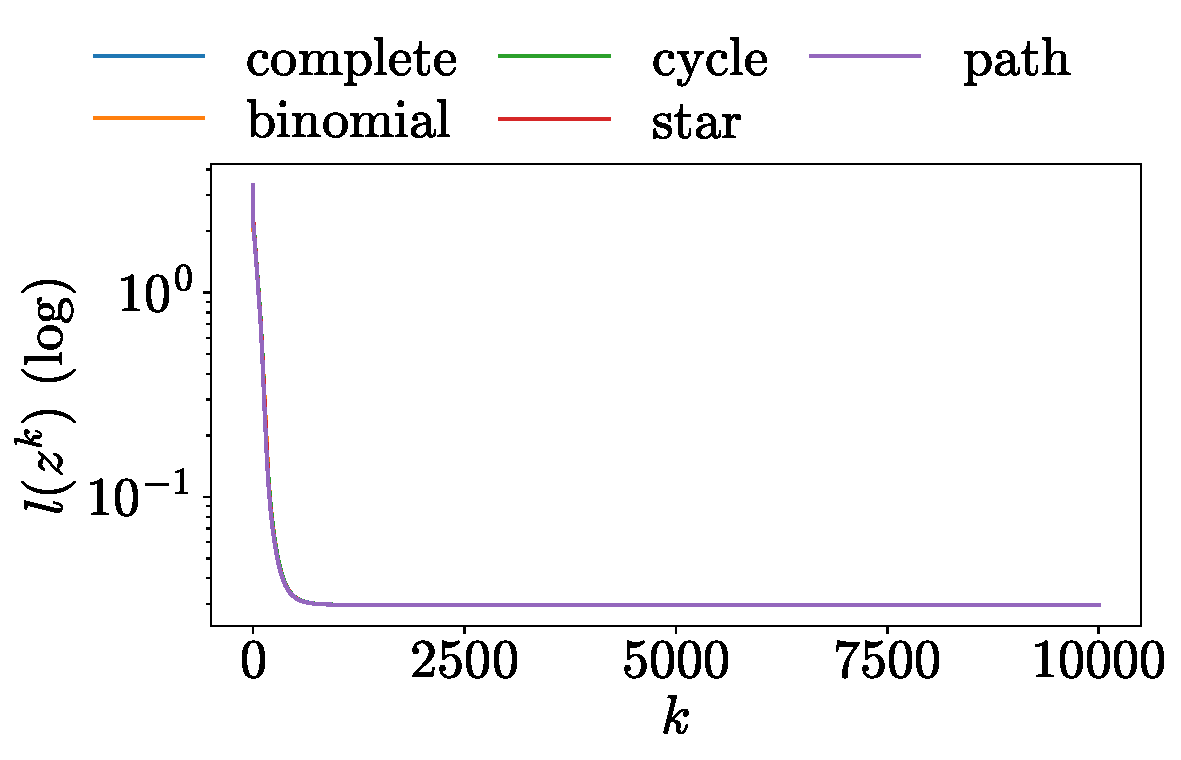
\includegraphics[width=\linewidth]{./figs/tracking/5_3_2/loss.pdf} 
            \caption{Loss evolution}
      \end{subfigure}
      \hfill
      \begin{subfigure}[h]{0.4\linewidth}
            \centering
            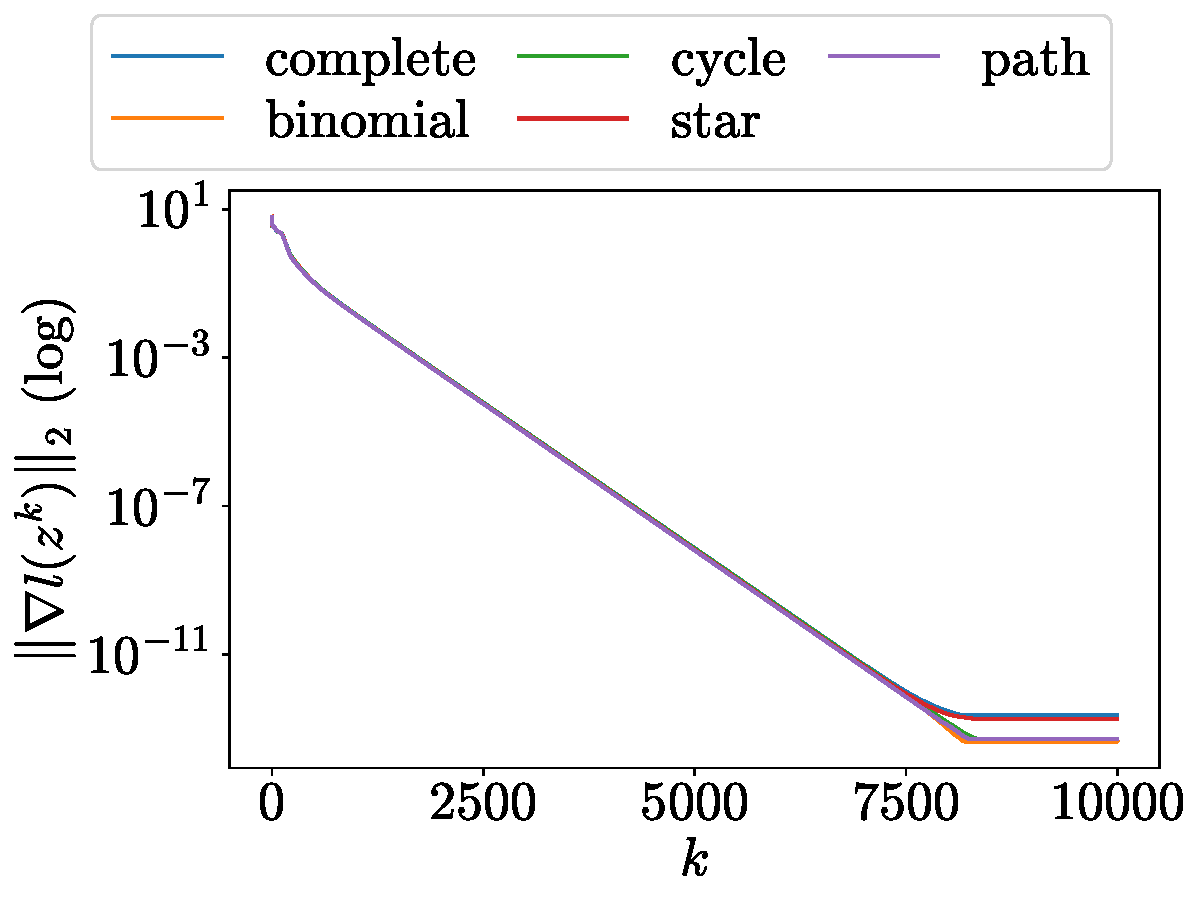
\includegraphics[width=\linewidth]{./figs/tracking/5_3_2/gradient.pdf} 
            \caption{Gradient norm evolution}
      \end{subfigure}
      \caption{Tracking with $5$ robots and $3$ targets}
      \label{fig:tracking_5_3}
\end{figure}


Instead, by increasing the number of tracking robots, we can see from \Cref{fig:tracking_15_3,fig:tracking_30_3} that the plateau is reached in fewer number of iterations, which intuitively means that more tracking robots help in reaching a faster convergence. Moreover, we can also observe from these figures that, as we already mentioned, with less connected graphs convergence is affected negatively.

\begin{figure}[h!]
      \centering
      \begin{subfigure}[h]{0.4\linewidth}
            \centering
            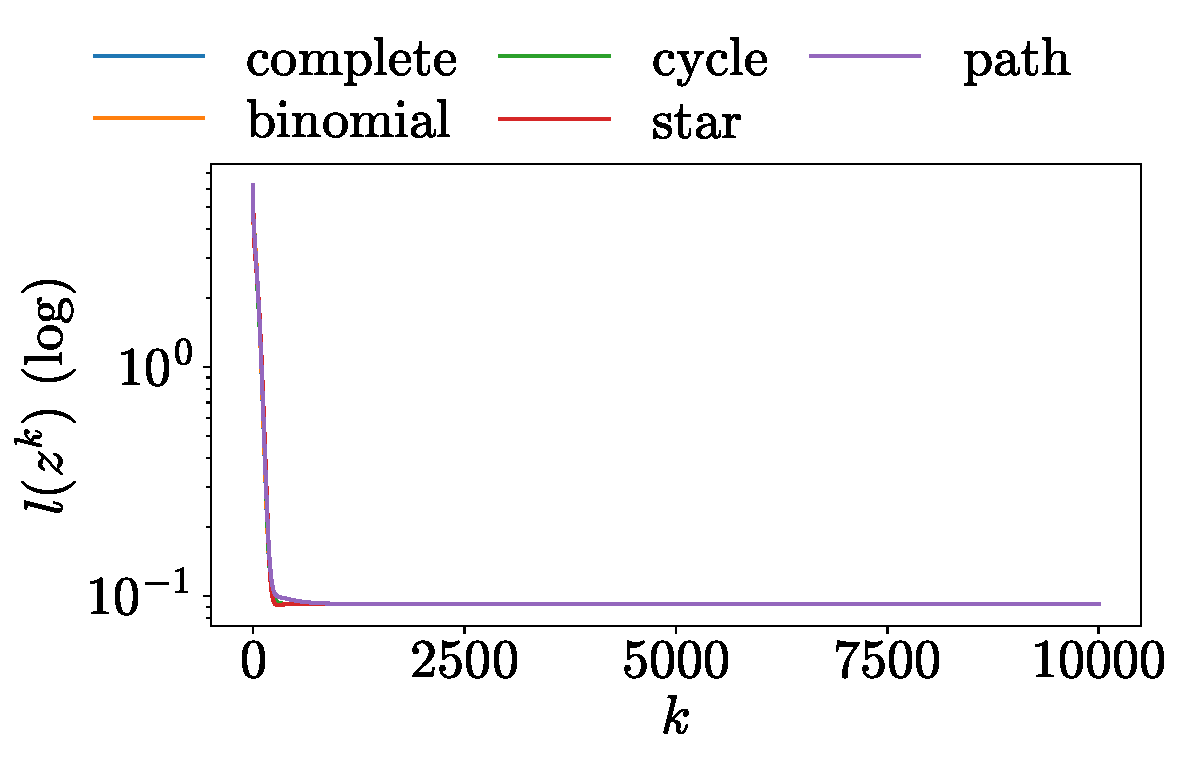
\includegraphics[width=\linewidth]{./figs/tracking/15_3_2/loss.pdf} 
            \caption{Loss evolution}
      \end{subfigure}
      \hfill
      \begin{subfigure}[h]{0.4\linewidth}
            \centering
            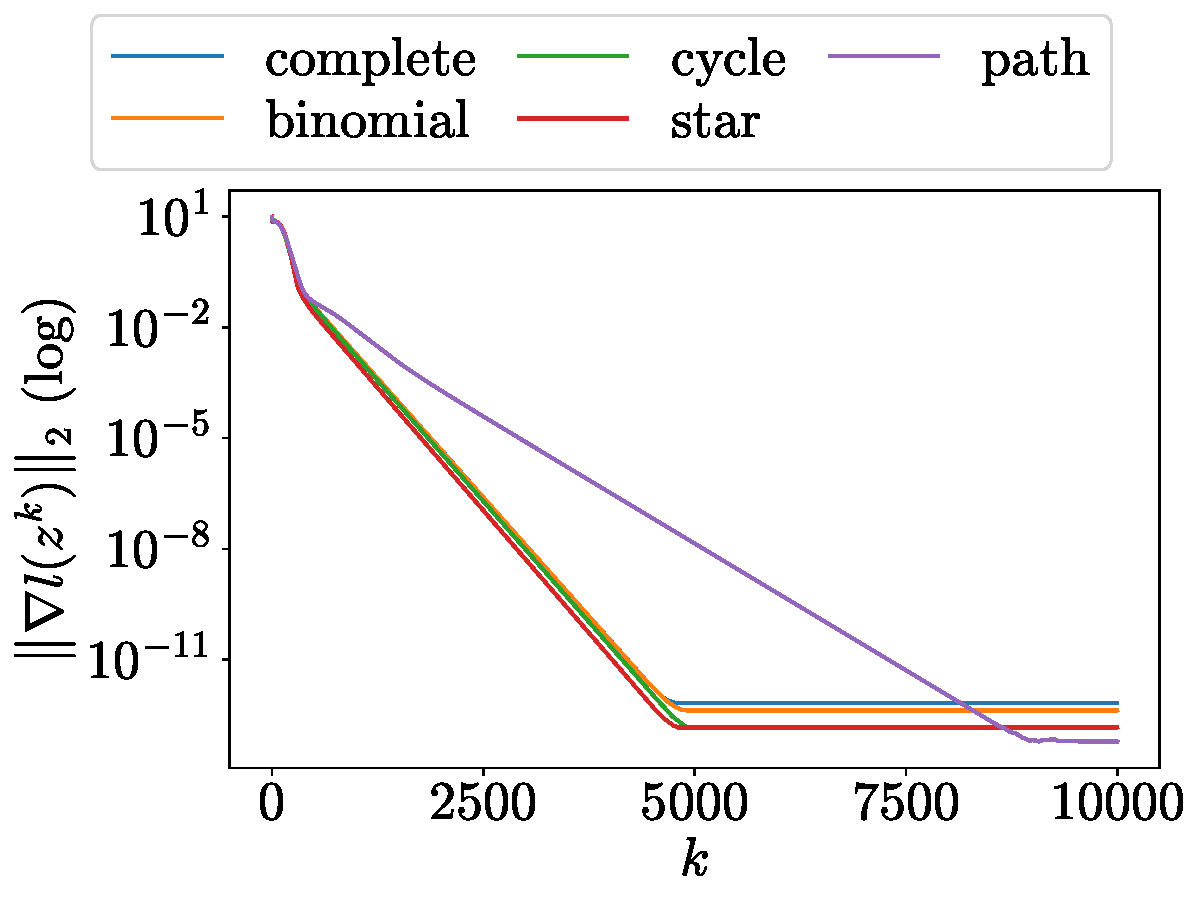
\includegraphics[width=\linewidth]{./figs/tracking/15_3_2/gradient.pdf} 
            \caption{Gradient norm evolution}
      \end{subfigure}
      \caption{Tracking with $15$ robots and $3$ targets}
      \label{fig:tracking_15_3}
\end{figure}

\begin{figure}[h!]
      \centering
      \begin{subfigure}[h]{0.4\linewidth}
            \centering
            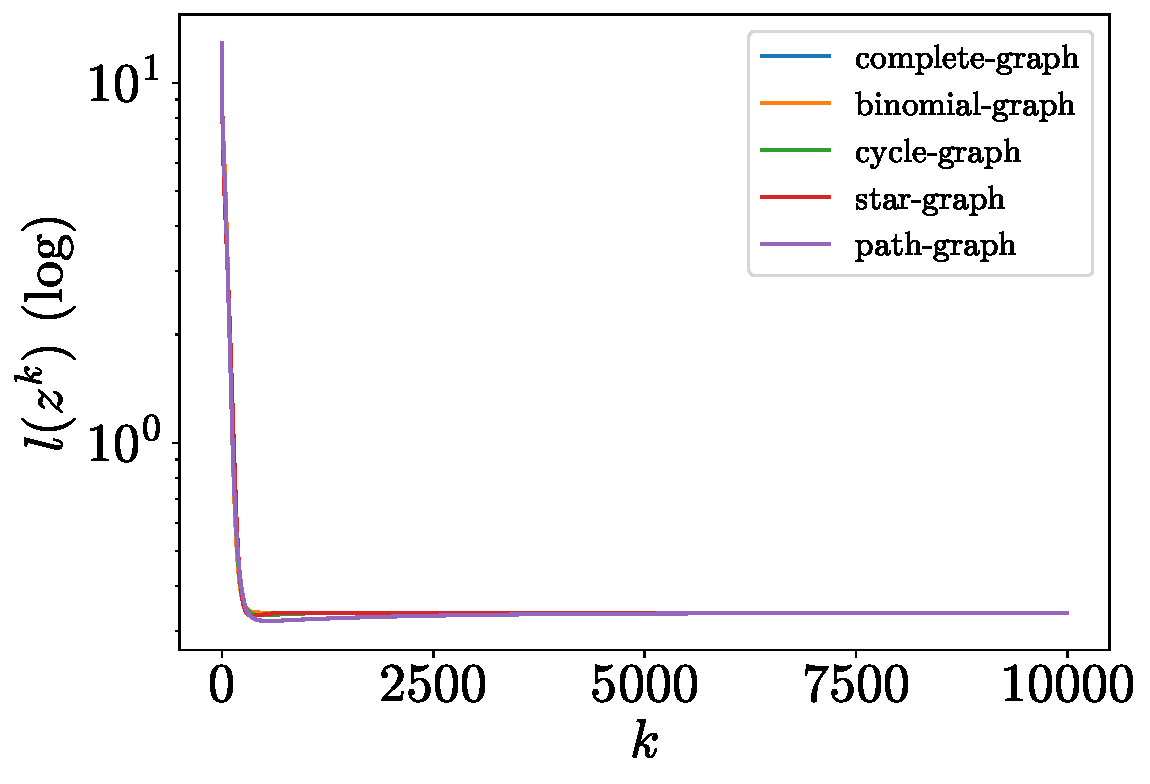
\includegraphics[width=\linewidth]{./figs/tracking/30_3_2/loss.pdf} 
            \caption{Loss evolution}
      \end{subfigure}
      \hfill
      \begin{subfigure}[h]{0.4\linewidth}
            \centering
            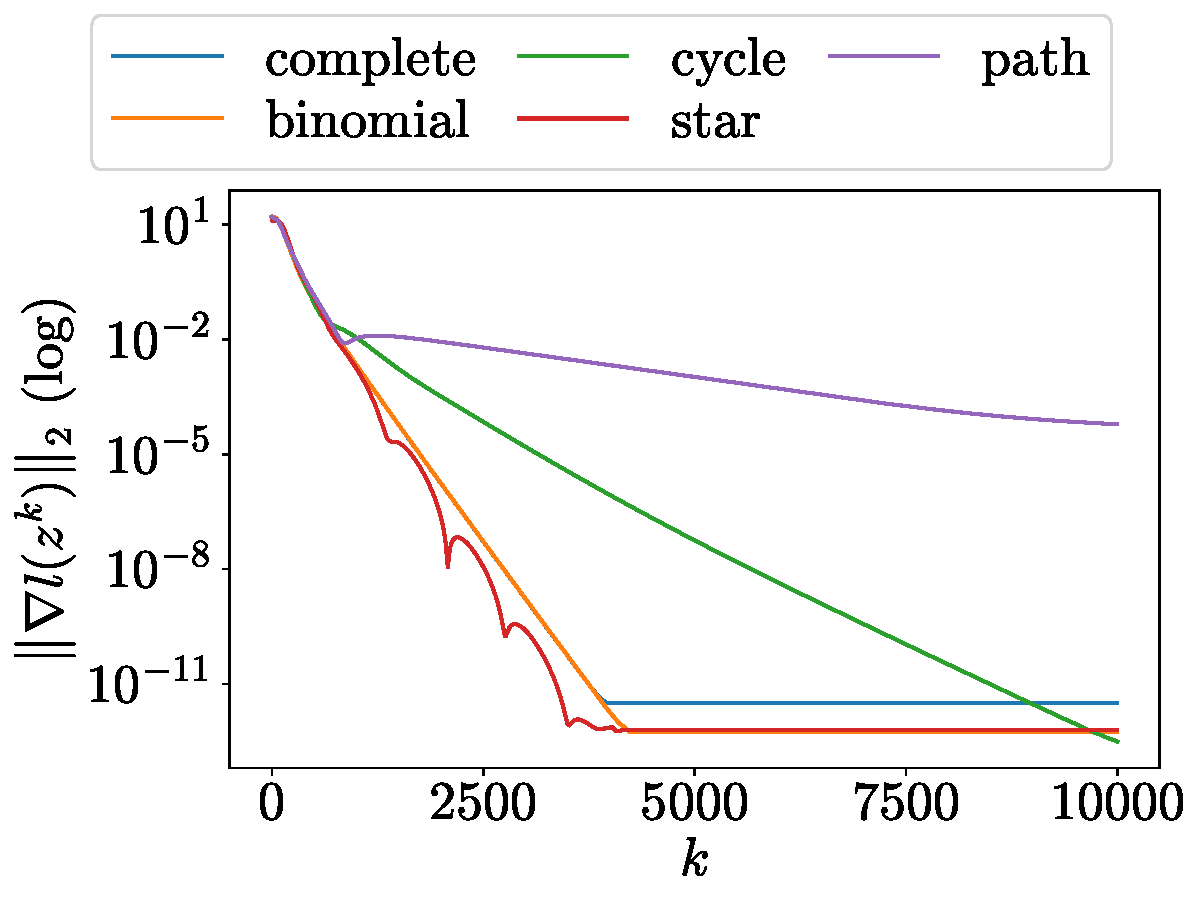
\includegraphics[width=\linewidth]{./figs/tracking/30_3_2/gradient.pdf} 
            \caption{Gradient norm evolution}
      \end{subfigure}
      \caption{Tracking with $30$ robots and $3$ targets}
      \label{fig:tracking_30_3}
\end{figure}


Moreover, as the total loss is a summation, we must note that the overall loss is higher in the case of more agents or targets, but this does not indicate worse tracking results. We report in \Cref{fig:tracking_avg_error_runs} the average distance over multiple runs between the estimated and real target positions for a fixed configuration with varying number of robots. It can be seen, as intuition would suggest, that on average the tracking error becomes smaller by increasing the number of tracking robots.

\begin{figure}[h!]
      \centering
      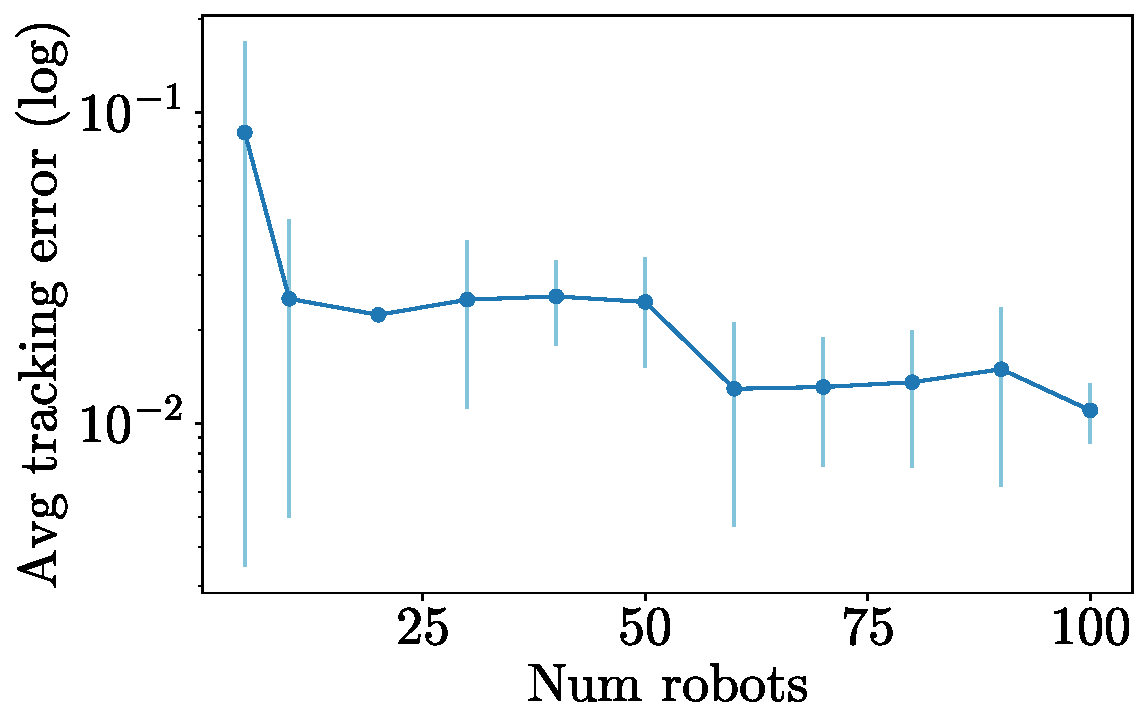
\includegraphics[width=0.46\linewidth]{./figs/tracking/average/avg_tracking.pdf}
      \caption{Average tracking error for different number of robots (average of 5 runs). Vertical bars represent the standard deviation.}
      \label{fig:tracking_avg_error_runs}
\end{figure}


Finally, an observation consistent in all experiments is that, as shown in \Cref{fig:tracking_consensus}, the overall behavior of this system is to reach an approximate consensus (i.e., consensus error around $10^{-4}$) in the first few iterations and then optimize the loss while improving and preserving consensus. This can also be observed in \Cref{fig:tracking_animation} where some frames of the animation of the scenario are shown.

\begin{figure}[h!]
      \centering
      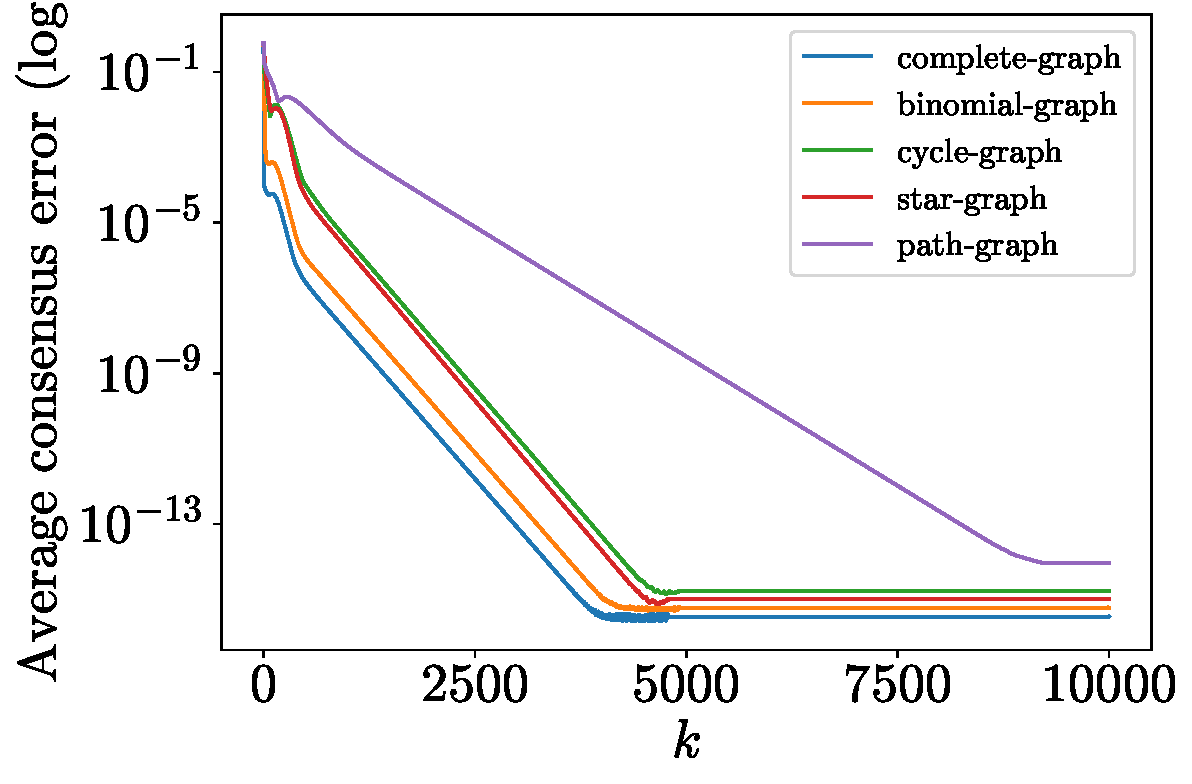
\includegraphics[width=0.44\linewidth]{./figs/tracking/15_3_2/consensus.pdf} 
      \caption{Tracking with $15$ robots and $3$ targets}
      \label{fig:tracking_consensus}
\end{figure}

\begin{figure}[h!]
      \centering
      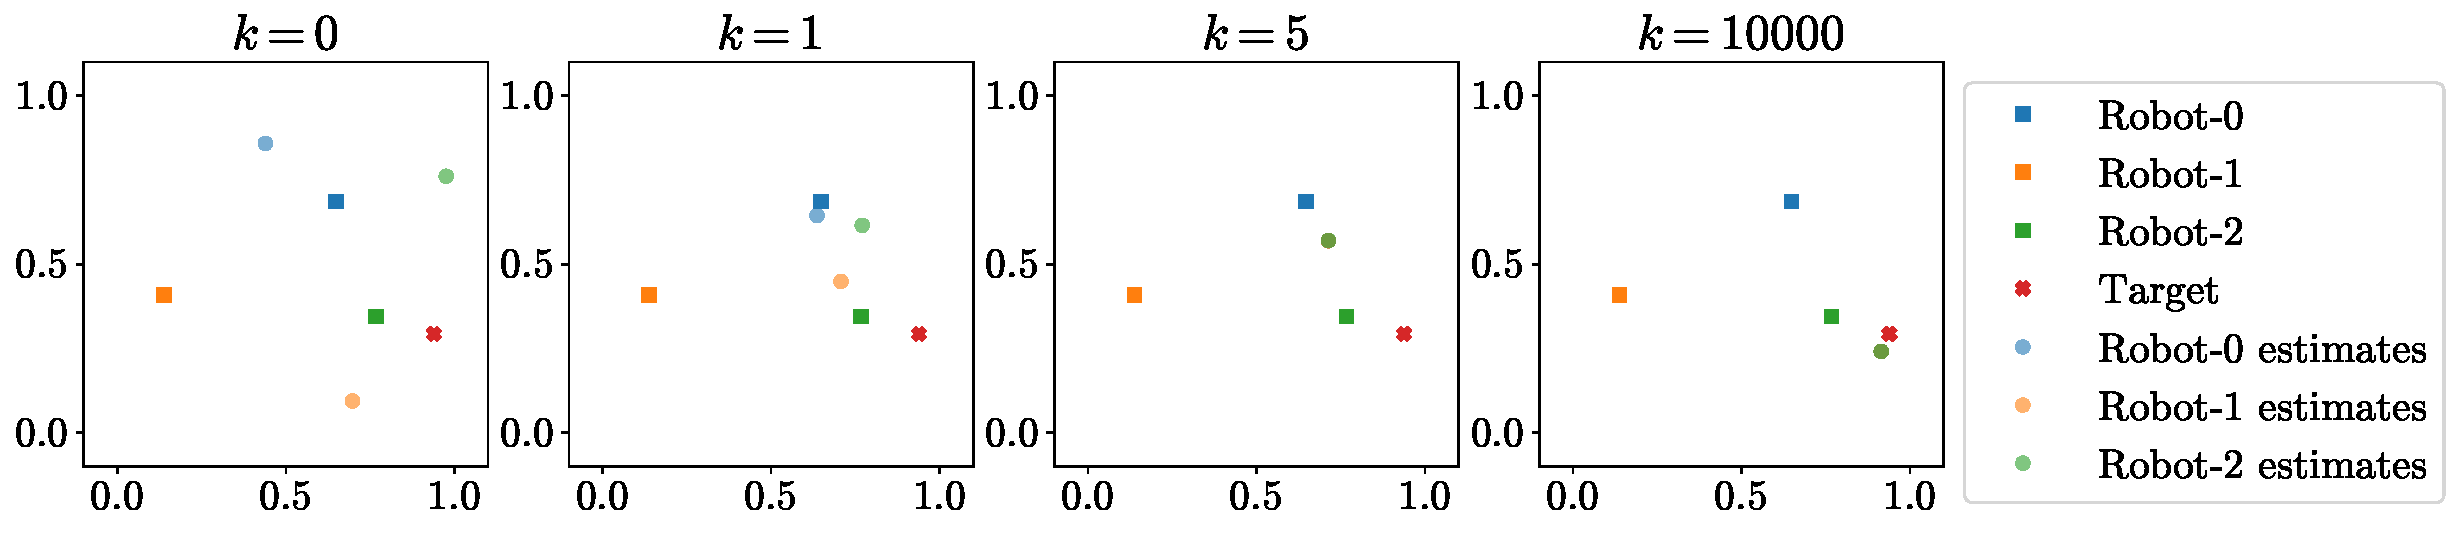
\includegraphics[width=0.9\linewidth]{./figs/tracking/anim.pdf} 
      \caption{Tracking animation with $3$ robots and $1$ target}
      \label{fig:tracking_animation}
\end{figure}


\subsection{Comparison with centralized gradient}

Compared with the centralized gradient algorithm, the plots in \Cref{fig:tracking_centralized_5_3} confirm what we observed before in the case of quadratic functions. The convergence speed is faster and more accurate in a centralized approach, which also results in a lower average tracking error.

\begin{figure}[h!]
      \centering
      \begin{subfigure}[h]{0.43\linewidth}
            \centering
            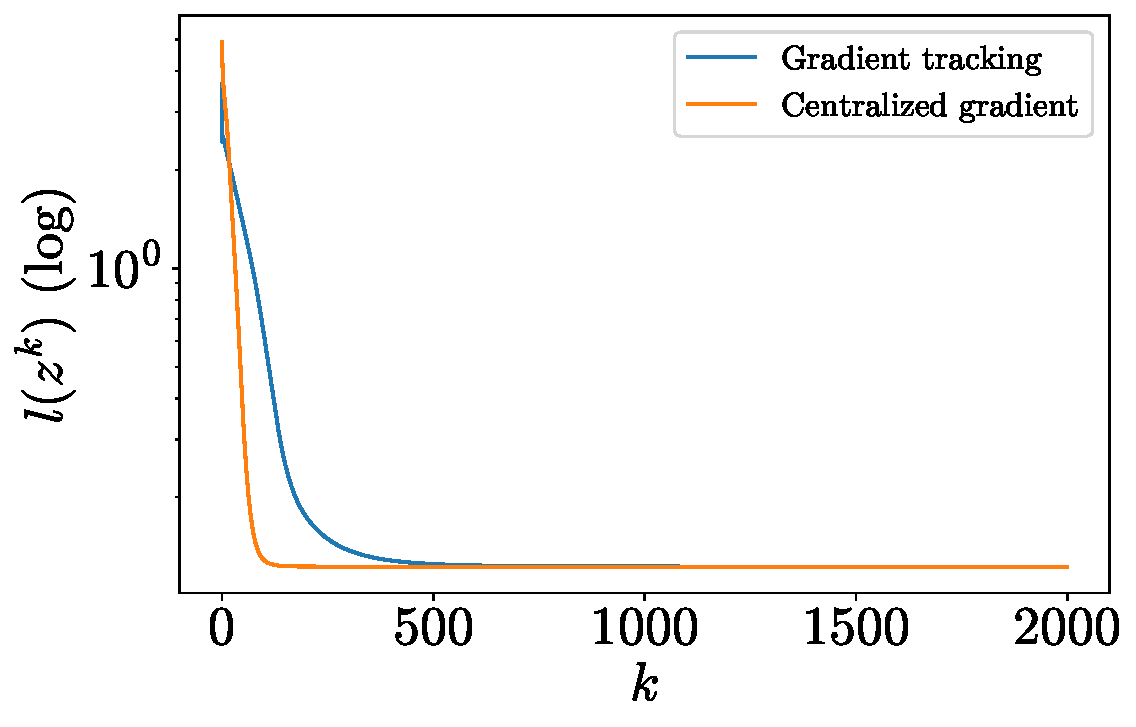
\includegraphics[width=\linewidth]{./figs/tracking/centralized/loss.pdf} 
            \caption{Loss evolution}
      \end{subfigure}
      \hfill
      \begin{subfigure}[h]{0.43\linewidth}
            \centering
            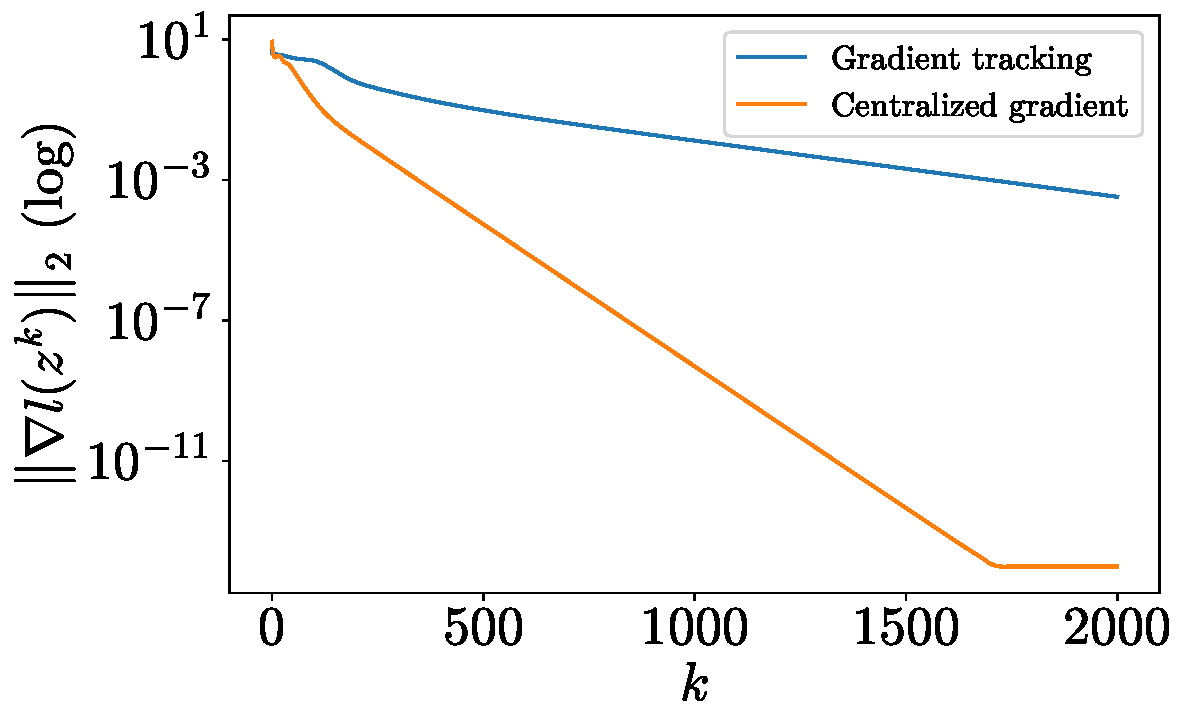
\includegraphics[width=\linewidth]{./figs/tracking/centralized/gradient.pdf} 
            \caption{Gradient norm evolution}
      \end{subfigure}
      \caption{Tracking with $15$ robots and $3$ targets compared to centralized gradient}
      \label{fig:tracking_centralized_5_3}
\end{figure}


\subsection{Comparison with different noises}

From the experiments with different noises, we observed a worsening in performance that is proportional to the amount of noise injected into the distance measurement, implying as one could expect that more noise leads to worse results. This behavior is consistent with noise drawn from different distributions as in \Cref{fig:tracking_gaussian_15_3,fig:tracking_poisson_15_3}, and also when the noise rate is increased as in \Cref{fig:tracking_rates_15_3}.

\begin{figure}[htb!]
      \centering
      \begin{subfigure}[h]{0.43\linewidth}
            \centering
            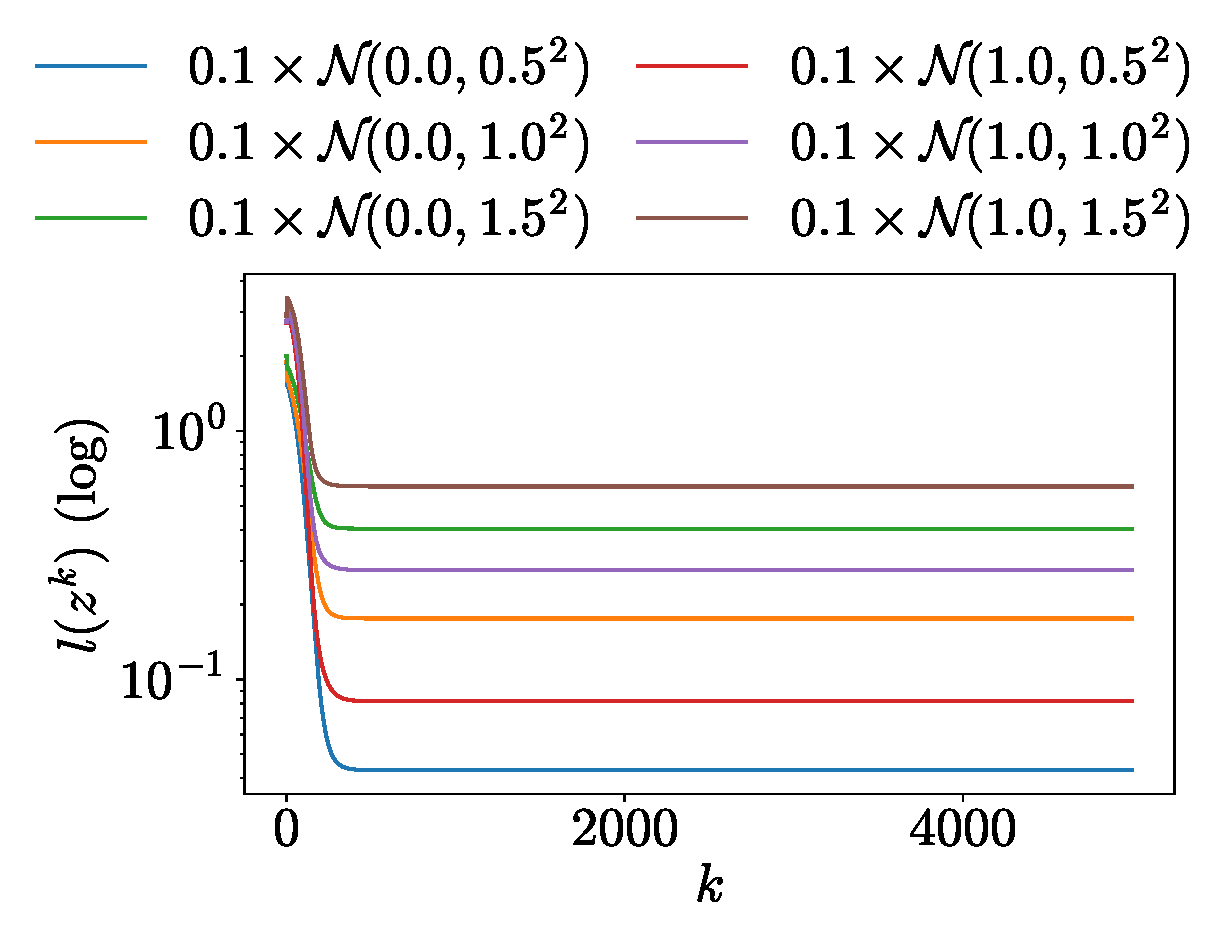
\includegraphics[width=\linewidth]{./figs/tracking/gaussian/loss.pdf} 
            \caption{Loss evolution}
      \end{subfigure}
      \hfill
      \begin{subfigure}[h]{0.43\linewidth}
            \centering
            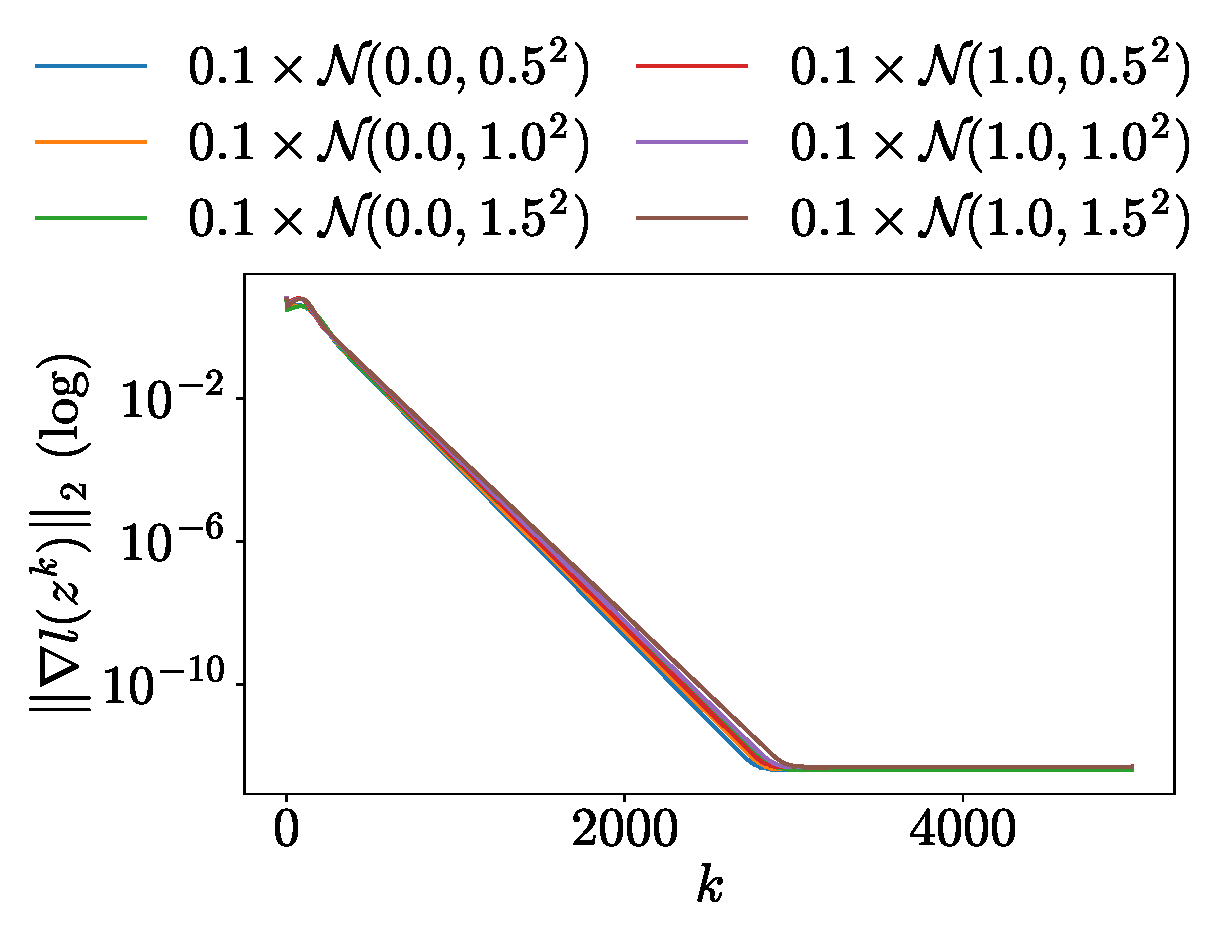
\includegraphics[width=\linewidth]{./figs/tracking/gaussian/gradient.pdf} 
            \caption{Gradient norm evolution}
      \end{subfigure}
      \caption{Tracking with $15$ robots and $3$ targets with noise drawn from Gaussian distributions}
      \label{fig:tracking_gaussian_15_3}
\end{figure}

\begin{figure}[H]
      \centering
      \begin{subfigure}[h]{0.43\linewidth}
            \centering
            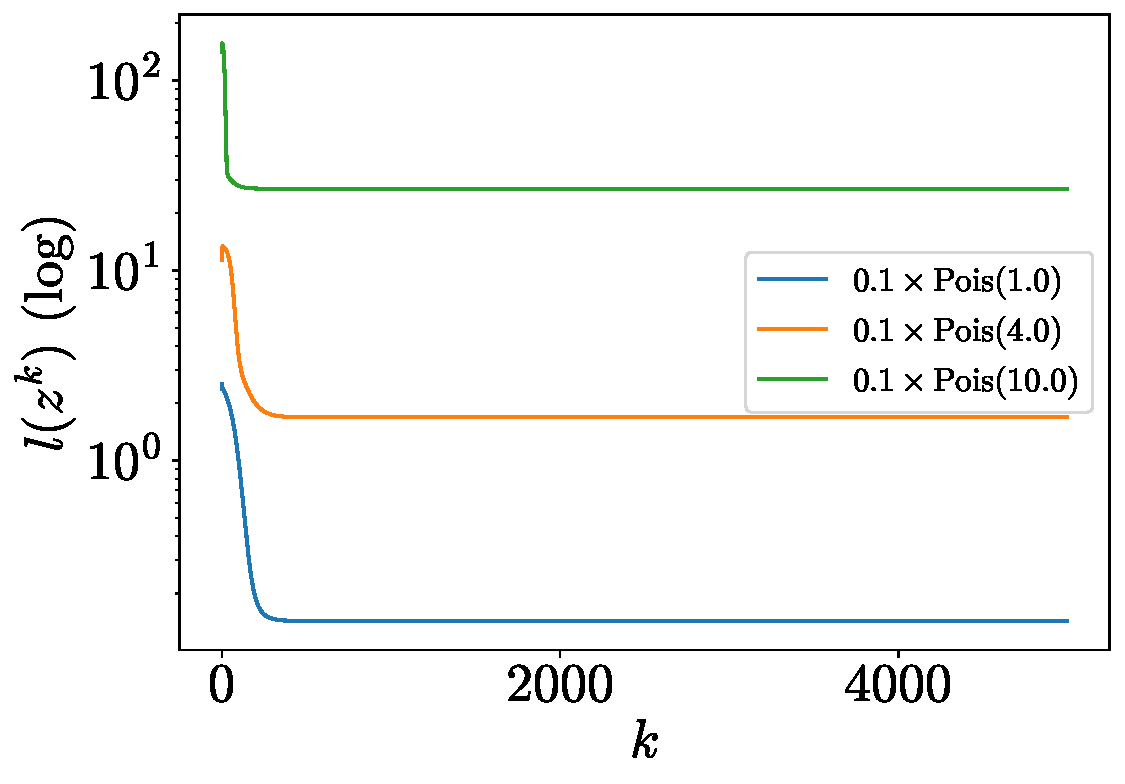
\includegraphics[width=\linewidth]{./figs/tracking/poisson/loss.pdf} 
            \caption{Loss evolution}
      \end{subfigure}
      \hfill
      \begin{subfigure}[h]{0.43\linewidth}
            \centering
            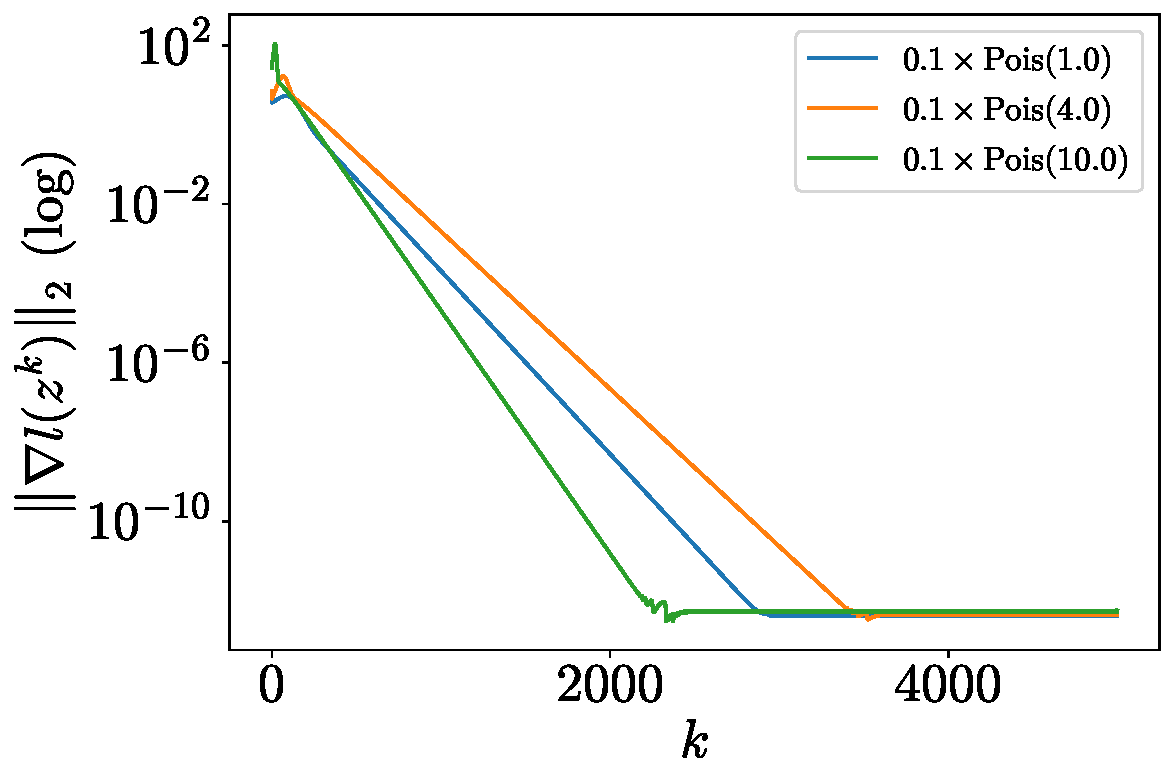
\includegraphics[width=\linewidth]{./figs/tracking/poisson/gradient.pdf} 
            \caption{Gradient norm evolution}
      \end{subfigure}
      \caption{Tracking with $15$ robots and $3$ targets with noise drawn from Poisson distributions}
      \label{fig:tracking_poisson_15_3}
\end{figure}

\begin{figure}[H]
      \centering
      \begin{subfigure}[h]{0.43\linewidth}
            \centering
            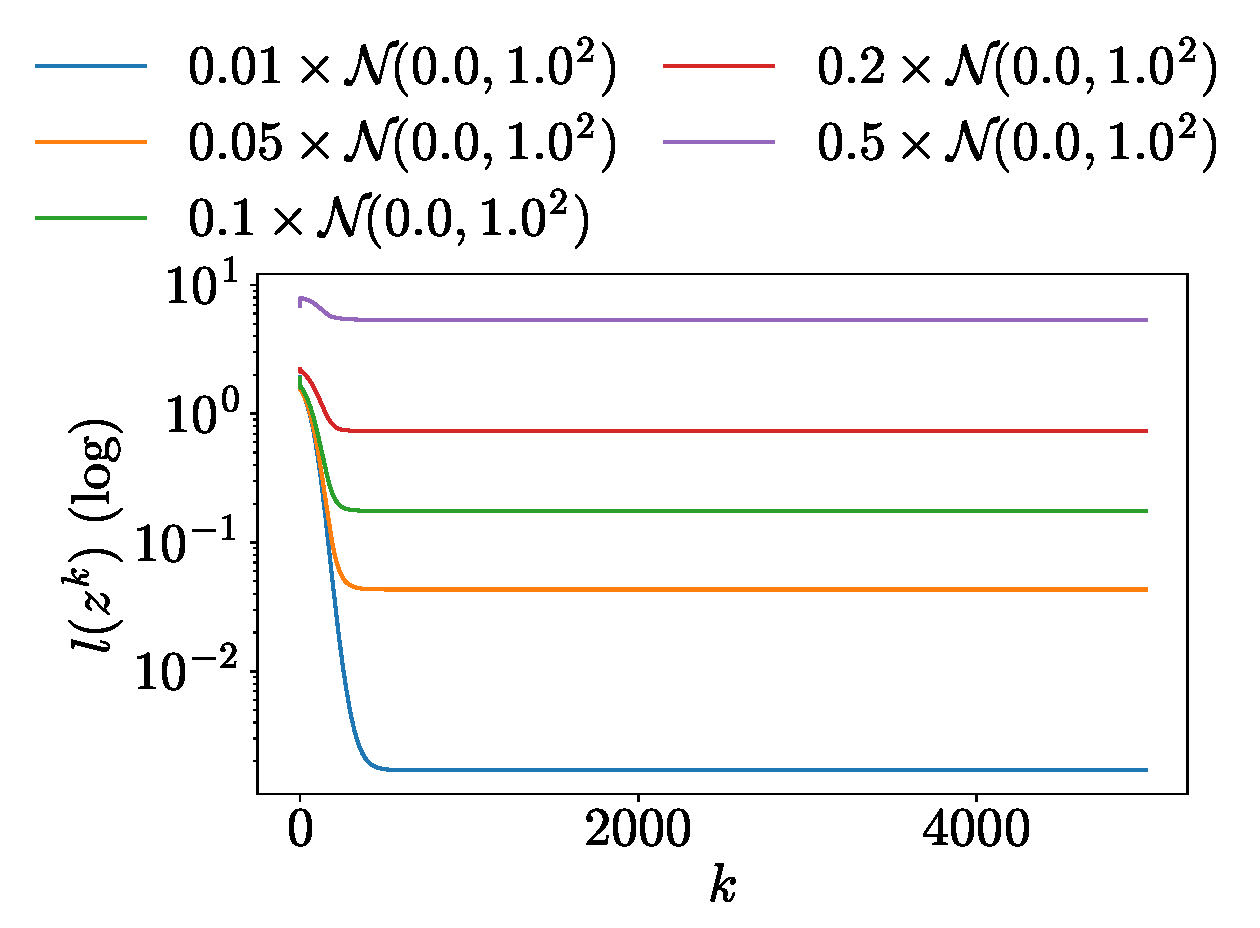
\includegraphics[width=\linewidth]{./figs/tracking/rates/loss.pdf} 
            \caption{Loss evolution}
      \end{subfigure}
      \hfill
      \begin{subfigure}[h]{0.43\linewidth}
            \centering
            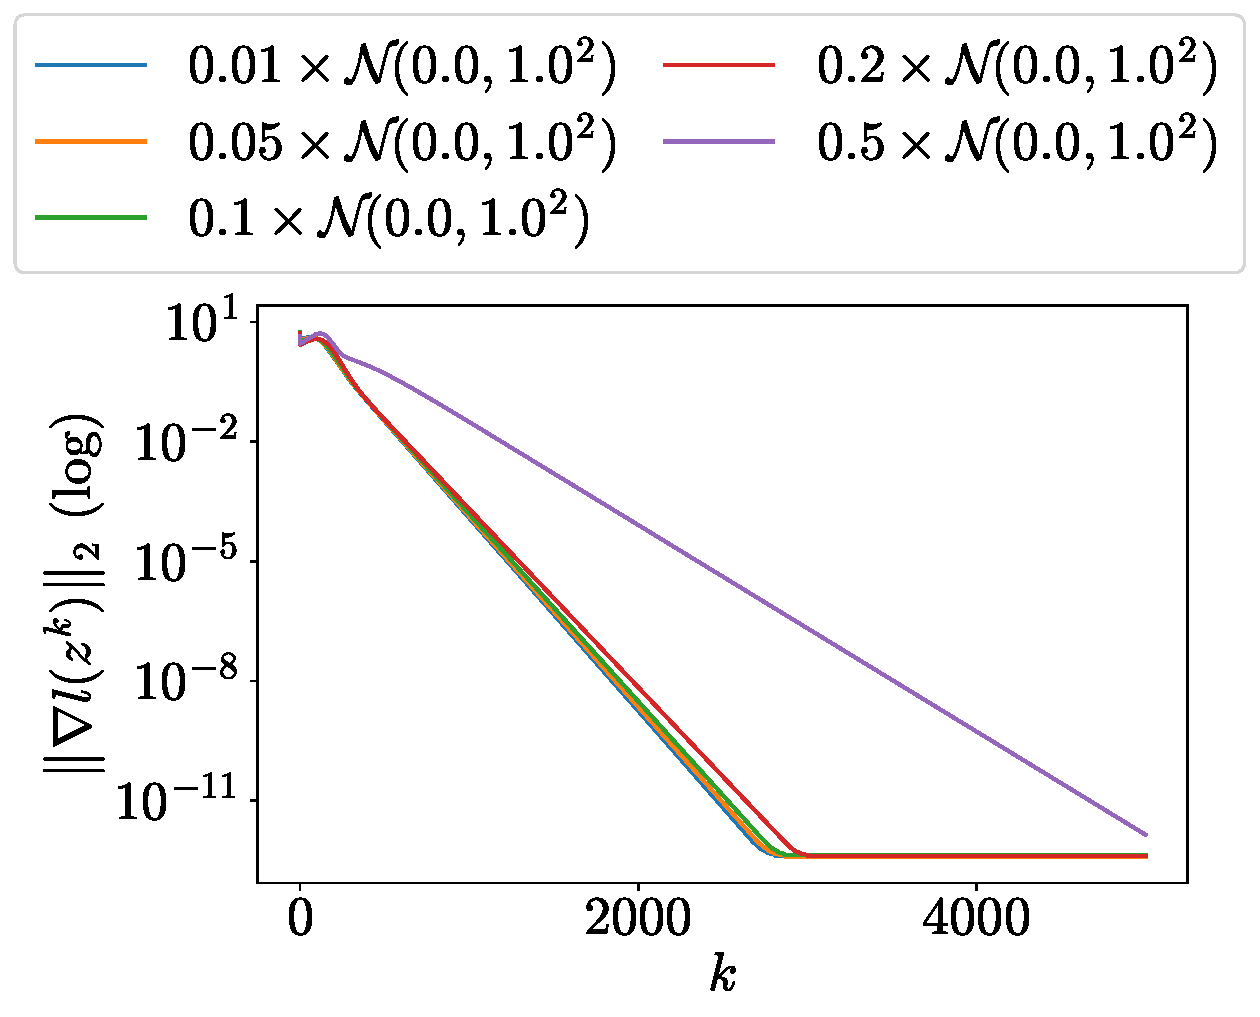
\includegraphics[width=\linewidth]{./figs/tracking/rates/gradient.pdf} 
            \caption{Gradient norm evolution}
      \end{subfigure}
      \caption{Tracking with $15$ robots and $3$ targets with different rates of Gaussian noise}
      \label{fig:tracking_rates_15_3}
\end{figure}




\chapter{Aggregative Optimization for Multi-Robot Systems} \label{ch:aggregative}



\section{Problem definition}

This task consists of solving the problem of positioning $N \in \N$ robots with positions $\z_i \in R^2$, for $i=1, \dots, N$, in such a way that they are close to their own private target $\r_i \in \R^2$ while staying tight to the fleet. This problem can be tackled using aggregative optimization by solving the following problem:
\[
      \begin{gathered}
            \min_{\z \in \R^{2N}} \sum_{i=1}^{N} l_i(\z_i, \sigma(\z)) \\
            \text{with } \sigma(\z) = \frac{1}{N} \sum_{i=1}^{N} \phi_i(\z_i),
      \end{gathered}
\]
where $\z=(\z_1, \dots, \z_N) \in \R^{2N}$ is the stack of the robots' positions, $l_i: \R^{2} \times \R^{2N} \rightarrow \R$ is the local loss of agent $i$, and $\sigma: \R^{2N} \rightarrow \R^2$ is an aggregation function.

We formulate the local loss of an agent $i$ as the following function:
\[
      l_i(\z_i, \sigma(\z)) = \gamma_1 \frac{1}{2} \Vert \z_i - \r_i \Vert^2 + \gamma_2 \frac{1}{2} \Vert \z_i - \sigma(\z) \Vert^2,
\]
where the first term models the vicinity to the private targets while the second one represents the fleet tightness. To add more flexibility, the hyperparameters $\gamma_1 \in \R$ and $\gamma_2 \in \R$ have been introduced to allow weighing the two requirements differently. The gradients of the loss with respect to the first and second arguments, respectively, are the following:
\[
      \begin{split}
            \nabla_1 l_i(\z_i, \sigma(\z)) &= \gamma_1 (\z_i - \r_i) + \gamma_2 (\z_i - \sigma(\z)) \\
            \nabla_2 l_i(\z_i, \sigma(\z)) &= -\gamma_2 (\z_i - \sigma(\z)),
      \end{split}
\]

In terms of aggregation function $\sigma(\z)$, the local function $\phi_i$ associated to agent $i$ is defined as follows:
\[
      \phi_i(\z_i) = \alpha_i \z_i,
\]
where $\alpha_i \in \R$ is a hyperparameter that can be different for each agent. With $\alpha_i = 1$ for all $i$, we obtain the standard formulation of the problem in which $\sigma(\z)$ represents the barycenter of the fleet. With different $\alpha_i$ (subject to $\sum_i^N \alpha_i = N$), we obtain a $\sigma(\z)$ that is a weighted average and can be interpreted as a barycenter that is biased towards specified agents.



\section{Code structure}
For the Python version, the code is structured with the following modules:
\begin{description}
      \item[\texttt{algorithm.py}] implements the aggregative optimization algorithm.
      \item[\texttt{loss.py}] contains the definition of the loss and the aggregative function.
      \item[\texttt{plot.py}] with the functions used to plot the loss, the gradient norm, and to animate the scenario.
      \item[\texttt{scenarios.py}] provides the functions to to create the communication graph and to initialize the parameters of the problem.
\end{description}
In practice all the experiments can be executed from the \texttt{main.py} script.

For the ROS2 version, the agent is implemented using the node defined in \texttt{Agent.py}. Each agent has a topic in which it publishes its states and it listens from the topics of its neighbors. A polling timer is used to control the communication frequency while the update steps are performed using the same functions defined in \texttt{algorithm.py}. For visualization, we implemented a node that acts as a middleware for RViz that reads from the topics of all agents and publishes some new topics for the specific markers that are visualized in RViz.



\section{Experiments}

As in the previous task, we first test the effectiveness of our implementation with different graph patterns for the communication graph and different number of agents. We test with configurations consisting of $5$, $15$, and $30$ robots. Then, to assess the actual results, we visually check the coherence of the positioning of the agents at convergence and experiment with different loss hyperparameters to favor specific agents, target vicinity, or fleet tightness.


\subsection{Comparison with different graph patterns}

We first test the implementation with $5$ agents. From the plots in \Cref{fig:positioning_5}, we can observe an identical trend in terms of loss and gradient for every graph pattern we have experimented with. In all cases, we can observe that, as expected from theoretical results, the algorithm converges.

\begin{figure}[h!]
      \centering
      \begin{subfigure}[h]{0.4\linewidth}
            \centering
            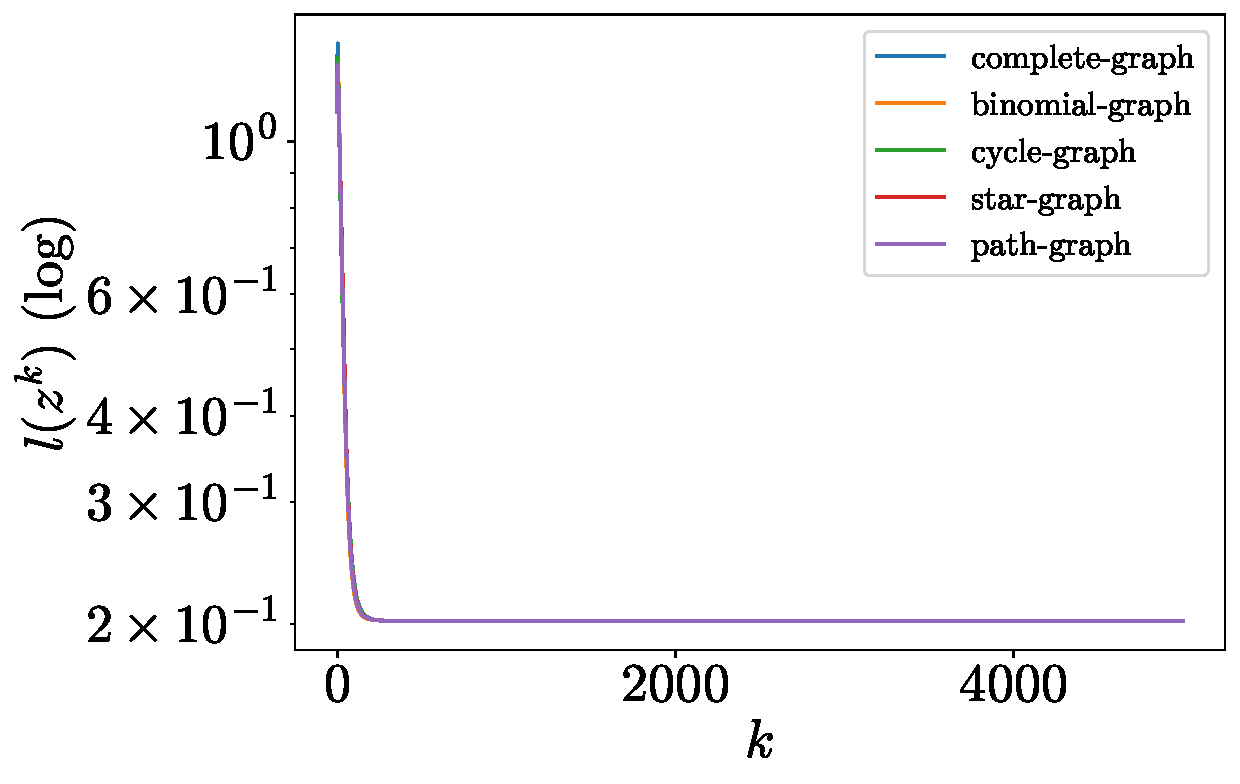
\includegraphics[width=\linewidth]{./figs/aggregative/few_agents/loss.pdf} 
            \caption{Loss evolution}
      \end{subfigure}
      \hfill
      \begin{subfigure}[h]{0.4\linewidth}
            \centering
            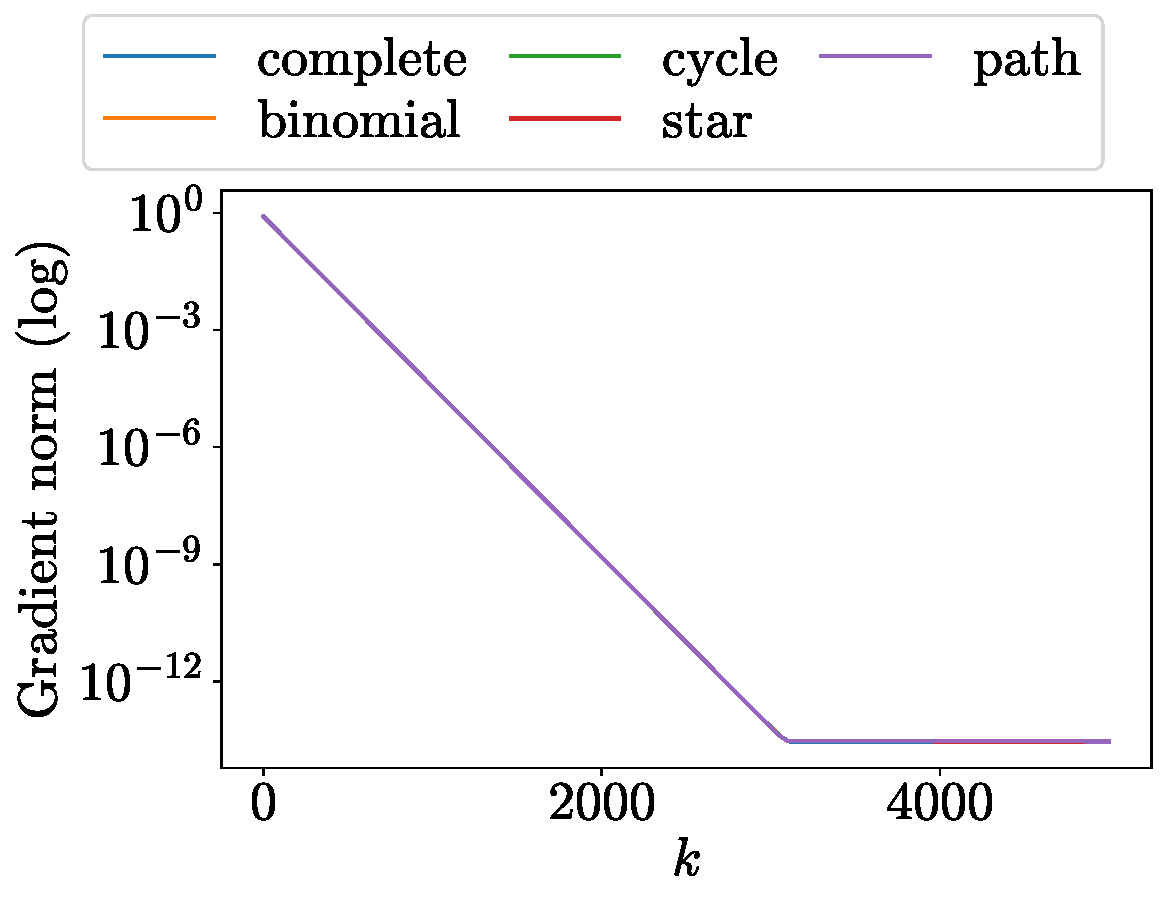
\includegraphics[width=\linewidth]{./figs/aggregative/few_agents/gradient.pdf} 
            \caption{Gradient norm evolution}
      \end{subfigure}
      \caption{Positioning with $5$ robots}
      \label{fig:positioning_5}
\end{figure}

\begin{figure}[h!]
      \centering
      \begin{subfigure}[h]{0.43\linewidth}
            \centering
            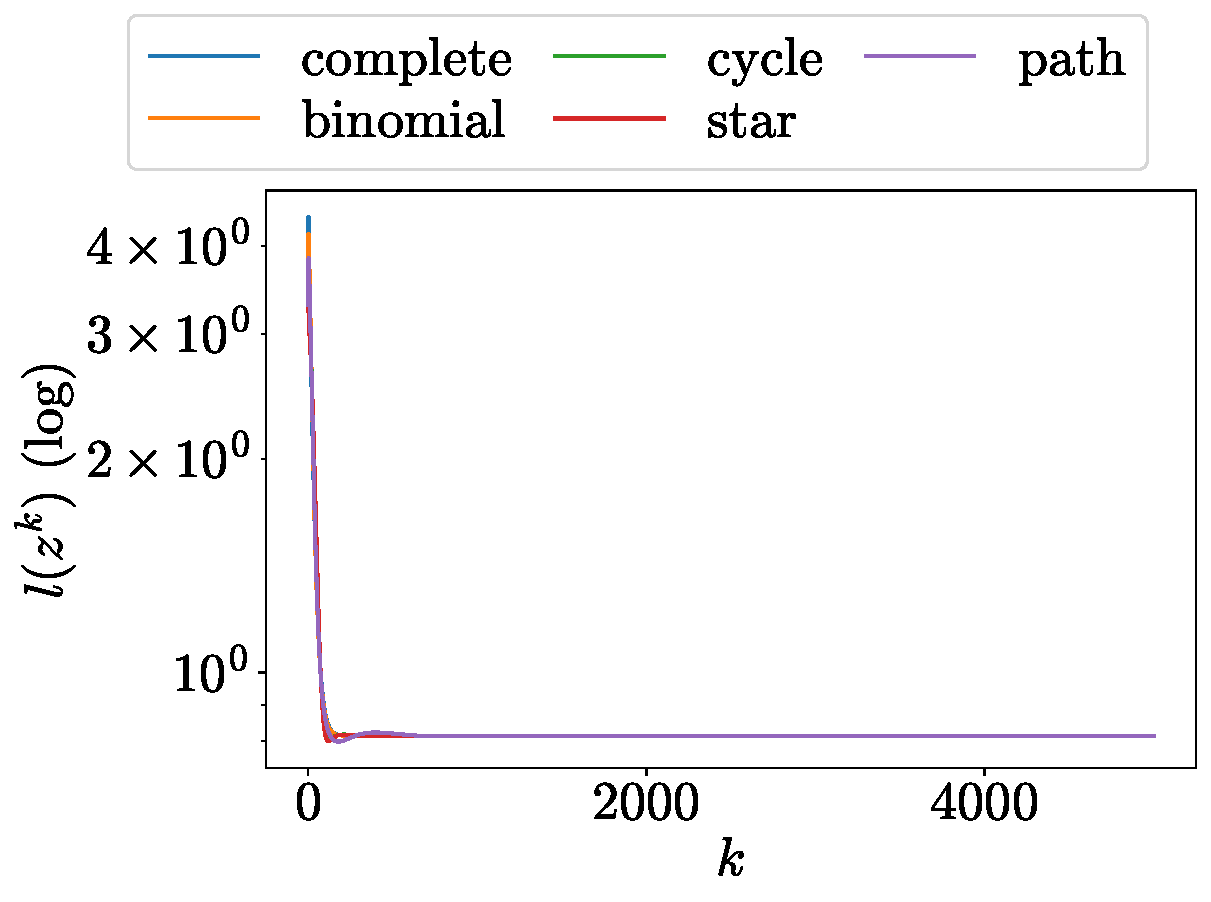
\includegraphics[width=\linewidth]{./figs/aggregative/more_agents/loss.pdf} 
            \caption{Loss evolution}
      \end{subfigure}
      \hfill
      \begin{subfigure}[h]{0.43\linewidth}
            \centering
            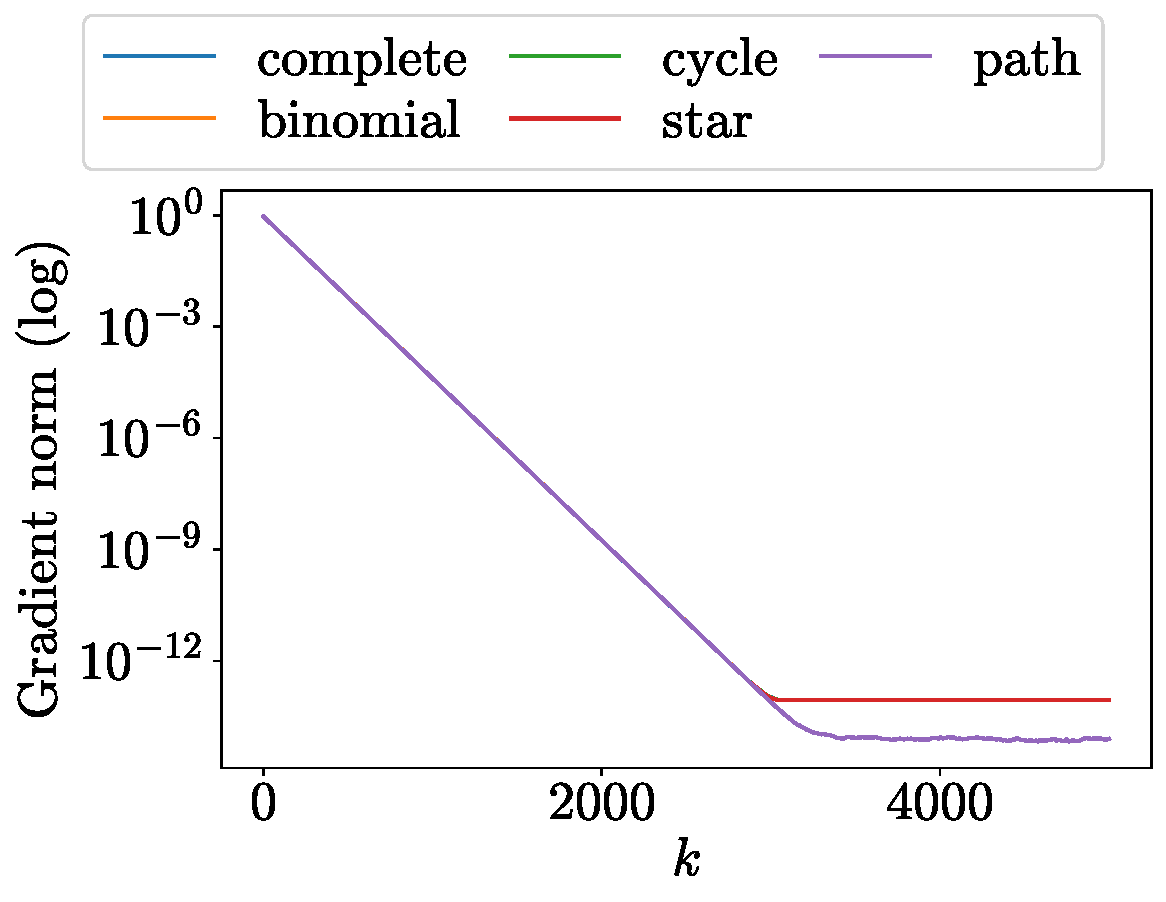
\includegraphics[width=\linewidth]{./figs/aggregative/more_agents/gradient.pdf} 
            \caption{Gradient norm evolution}
      \end{subfigure}
      \caption{Positioning with $15$ robots}
      \label{fig:positioning_15}
\end{figure}

\begin{figure}[h!]
      \centering
      \begin{subfigure}[h]{0.43\linewidth}
            \centering
            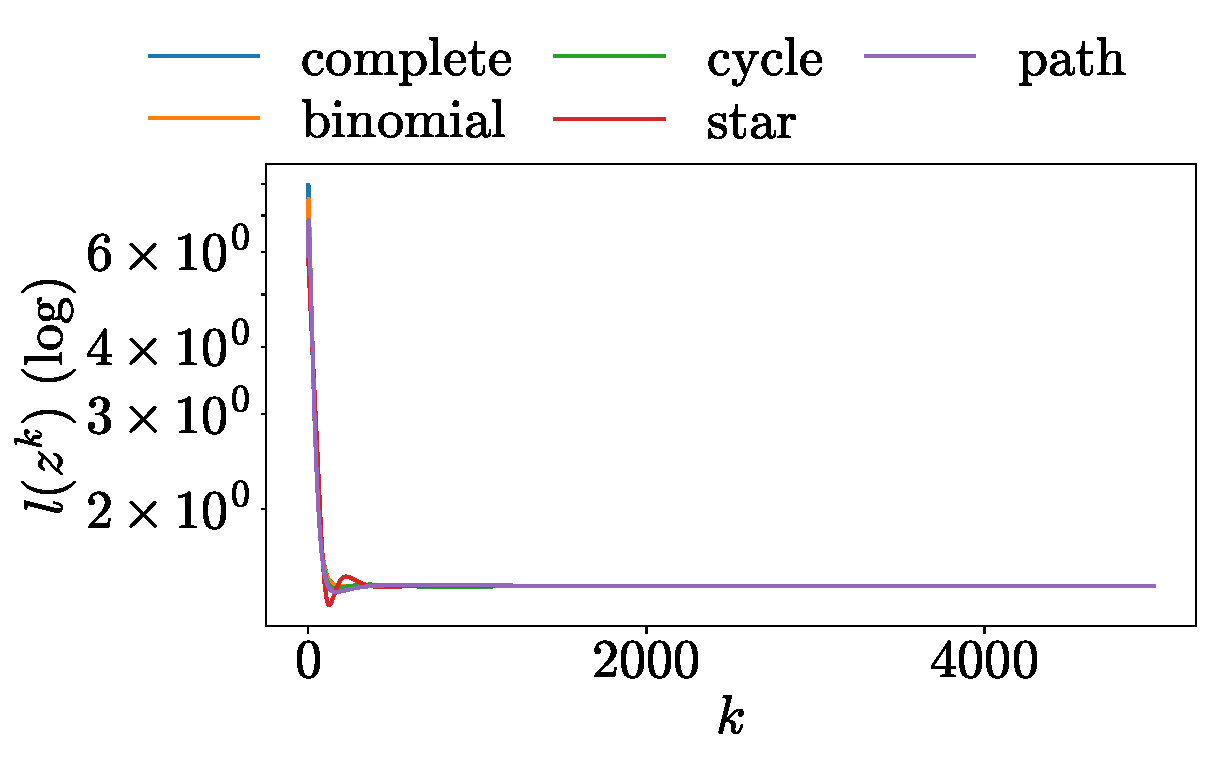
\includegraphics[width=\linewidth]{./figs/aggregative/lots_agents/loss.pdf} 
            \caption{Loss evolution}
      \end{subfigure}
      \hfill
      \begin{subfigure}[h]{0.4\linewidth}
            \centering
            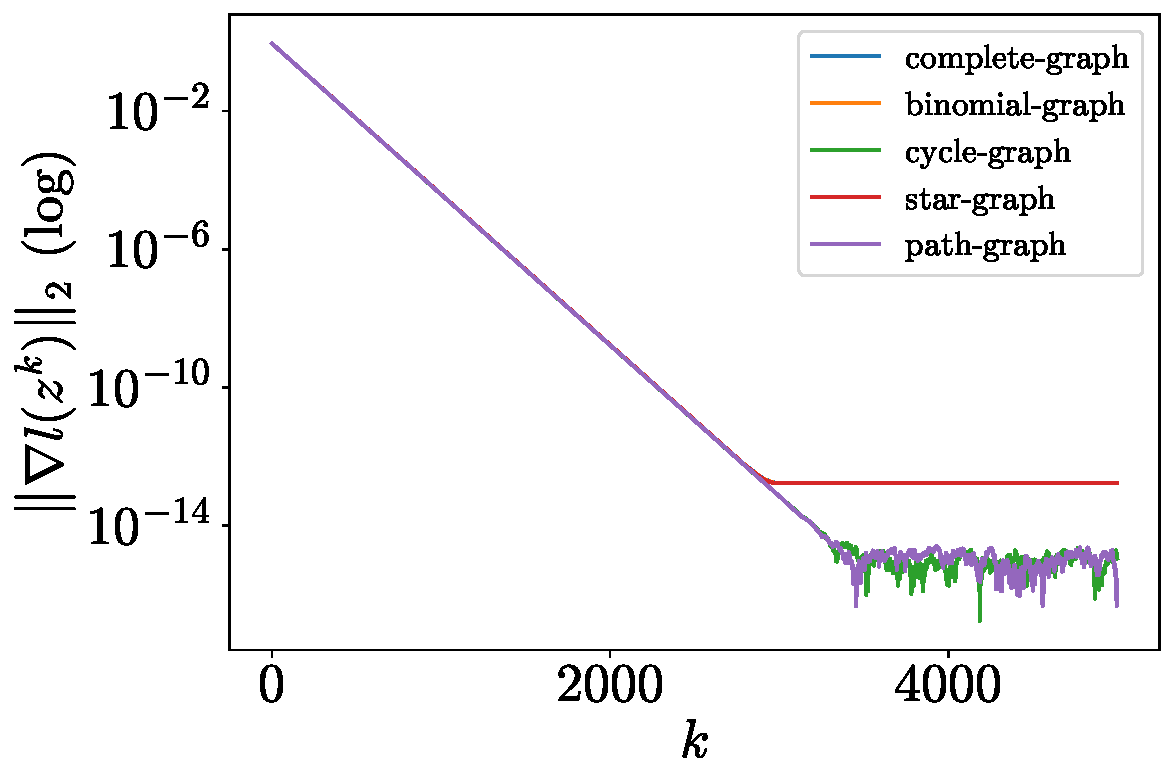
\includegraphics[width=\linewidth]{./figs/aggregative/lots_agents/gradient.pdf} 
            \caption{Gradient norm evolution}
      \end{subfigure}
      \caption{Positioning with $30$ robots}
      \label{fig:positioning_30}
\end{figure}

By considering a scenario with $15$ and $30$ agents, as shown in \Cref{fig:positioning_15,fig:positioning_30}, we cannot detect any relevant changes in behavior as they all reach convergence in a similar way as in the experiment with $5$ agents. The only thing we can underline is that the trend for less connected graphs have a little variation at convergence, most likely due to numerical instability.


\subsection{Comparison with different loss configurations}

To test the visual results, we first check the outcome in the plain version with equally weighted loss components and equal agents' importance. Results are presented in \Cref{fig:anim_plain} for Python and \Cref{fig:anim_plain_ros2} for ROS2. As one could expect, with the two components of the loss balanced, neither are favored and the agents converge to a position that is midway between the barycenter and their private target.
\begin{figure}[h!]
      \centering
      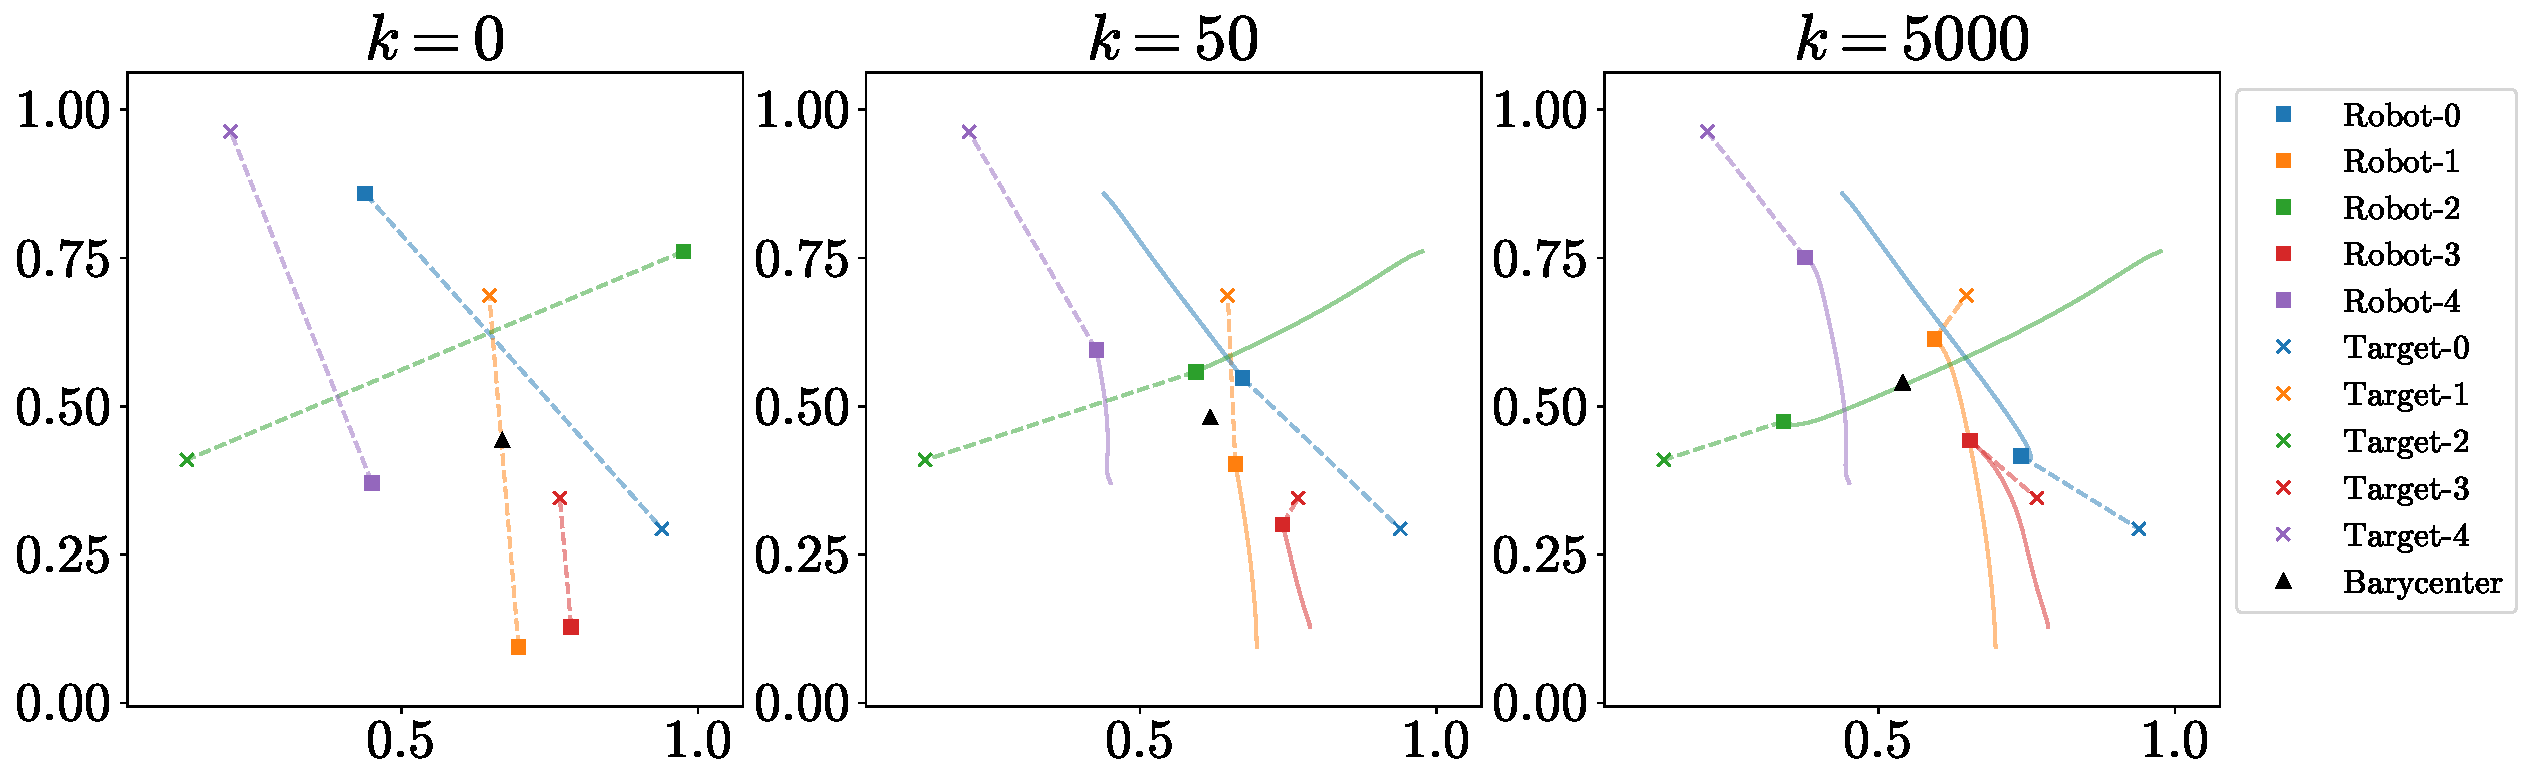
\includegraphics[width=0.9\linewidth]{./figs/aggregative/plain_anim/anim.pdf} 
      \caption{Frames with $5$ robots and balanced loss. Dashed lines connect robots to the targets and solid lines are the trajectories.}
      \label{fig:anim_plain}
\end{figure}

\begin{figure}[h!]
      \centering
      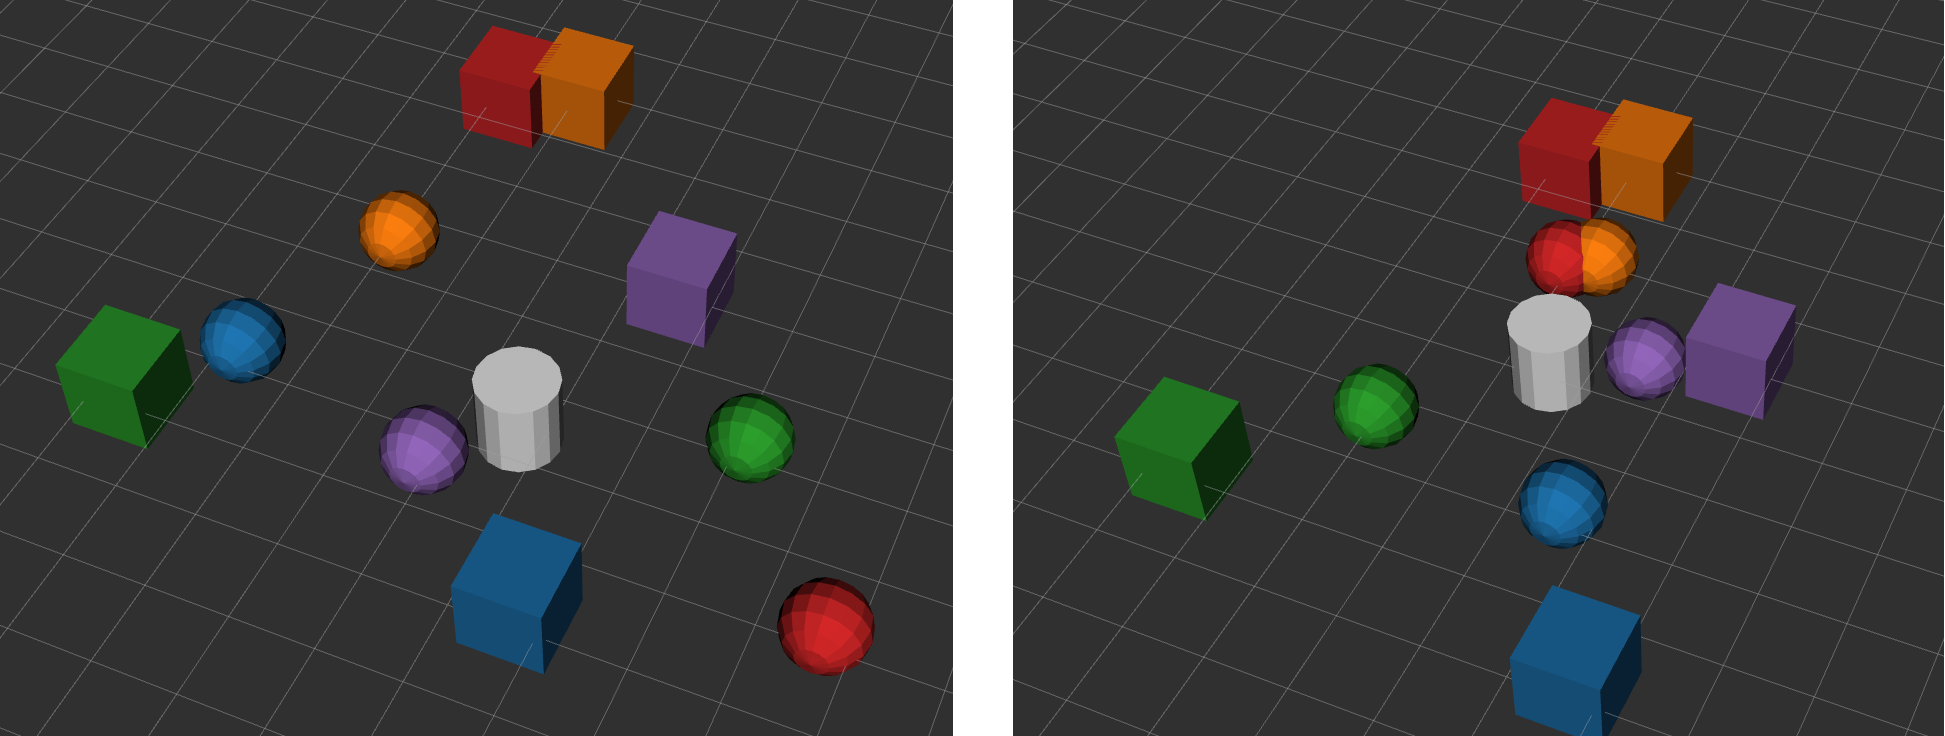
\includegraphics[width=0.75\linewidth]{./figs/aggregative/plain_anim/ros2.png} 
      \caption{Frames with $5$ robots and barycenter that prioritizes robot $0$. Spheres are agents, cubes are targets, and the cylinder is the barycenter.}
      \label{fig:anim_plain_ros2}
\end{figure}

Then, we continue the experiments by checking the results in terms of different loss hyperparameters. We experiment our formulation with different weights to prioritize target vicinity (higher $\gamma_1$), barycenter vicinity (higher $\gamma_2$), and different agents' importance (different $\alpha_i$). Results are presented in \Cref{fig:anim_target}, \Cref{fig:anim_barycenter}, and \Cref{fig:anim_importance}, respectively. In all cases the positions at convergence are intuitively the expected ones, showing that the algorithm allows many degrees of freedom.

\begin{figure}[H]
      \centering
      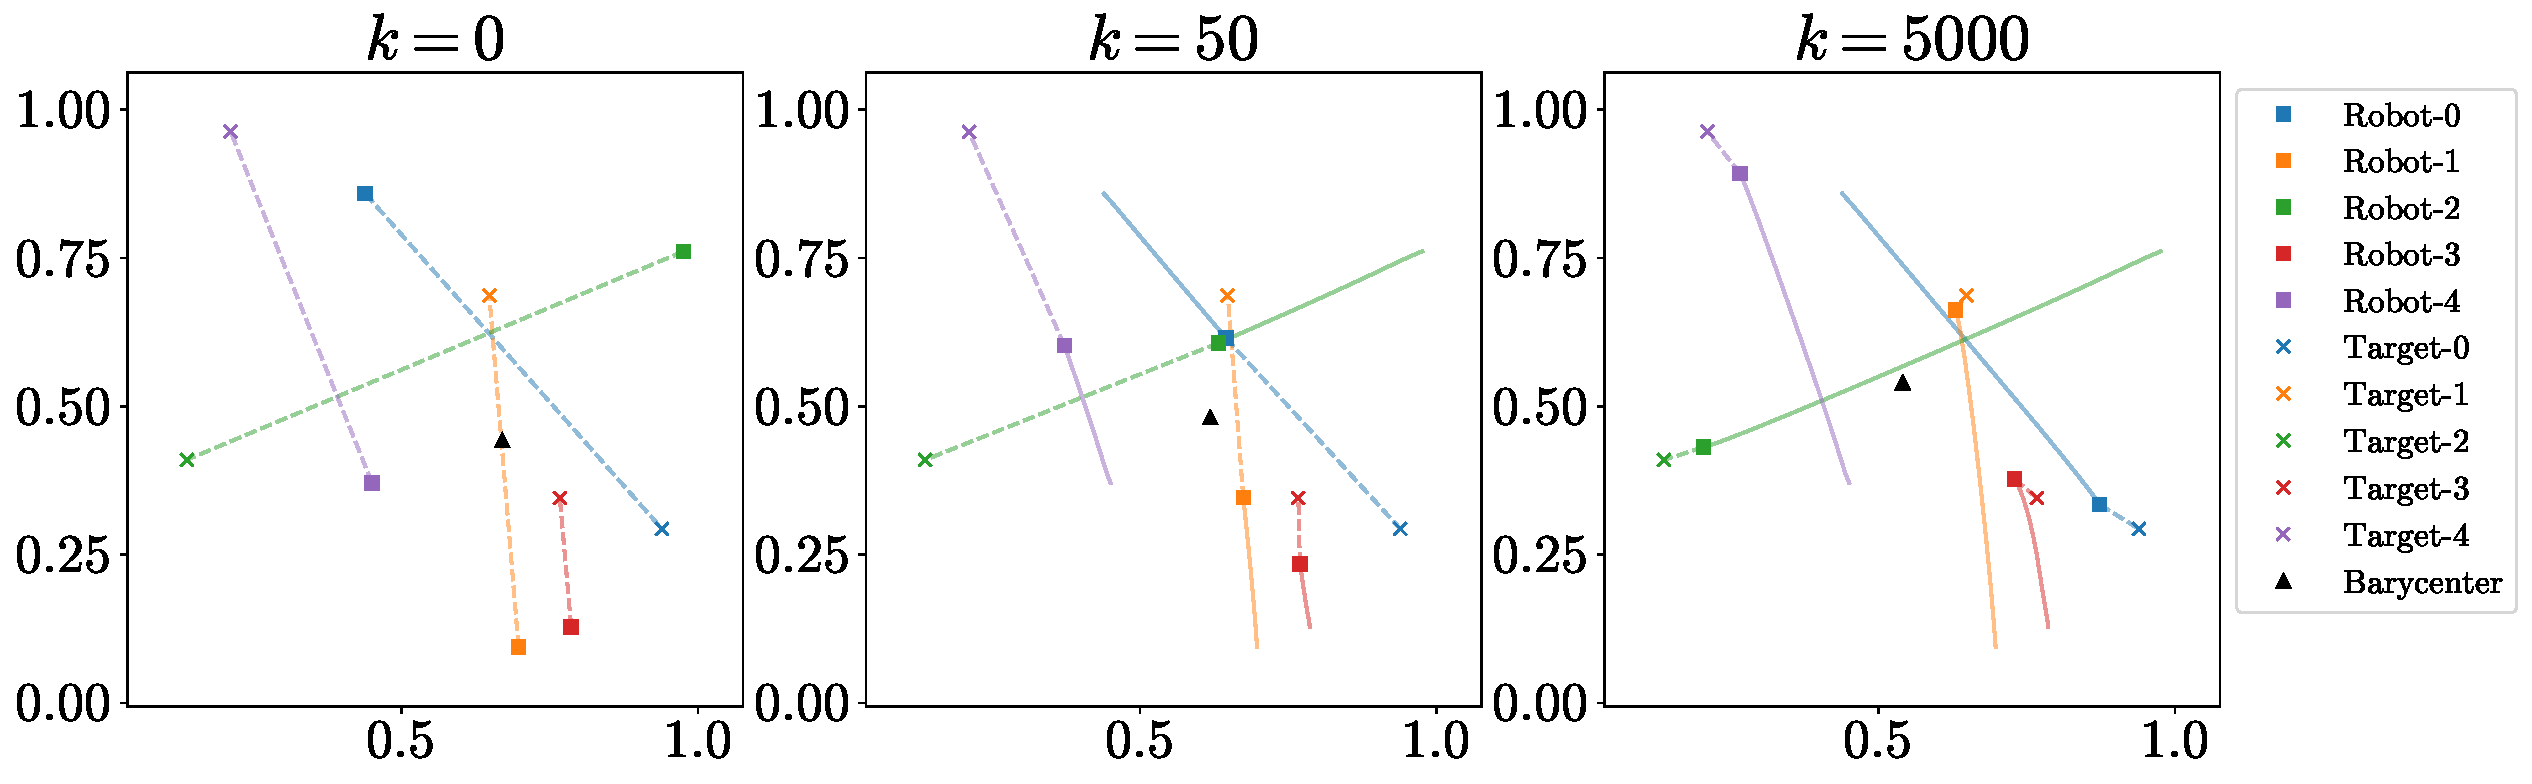
\includegraphics[width=0.9\linewidth]{./figs/aggregative/target_anim/anim.pdf} 
      \caption{Frames with $5$ robots and loss that prioritizes the private targets. Dashed lines connect robots to the targets and solid lines are the trajectories.}
      \label{fig:anim_target}
\end{figure}

\begin{figure}[H]
      \centering
      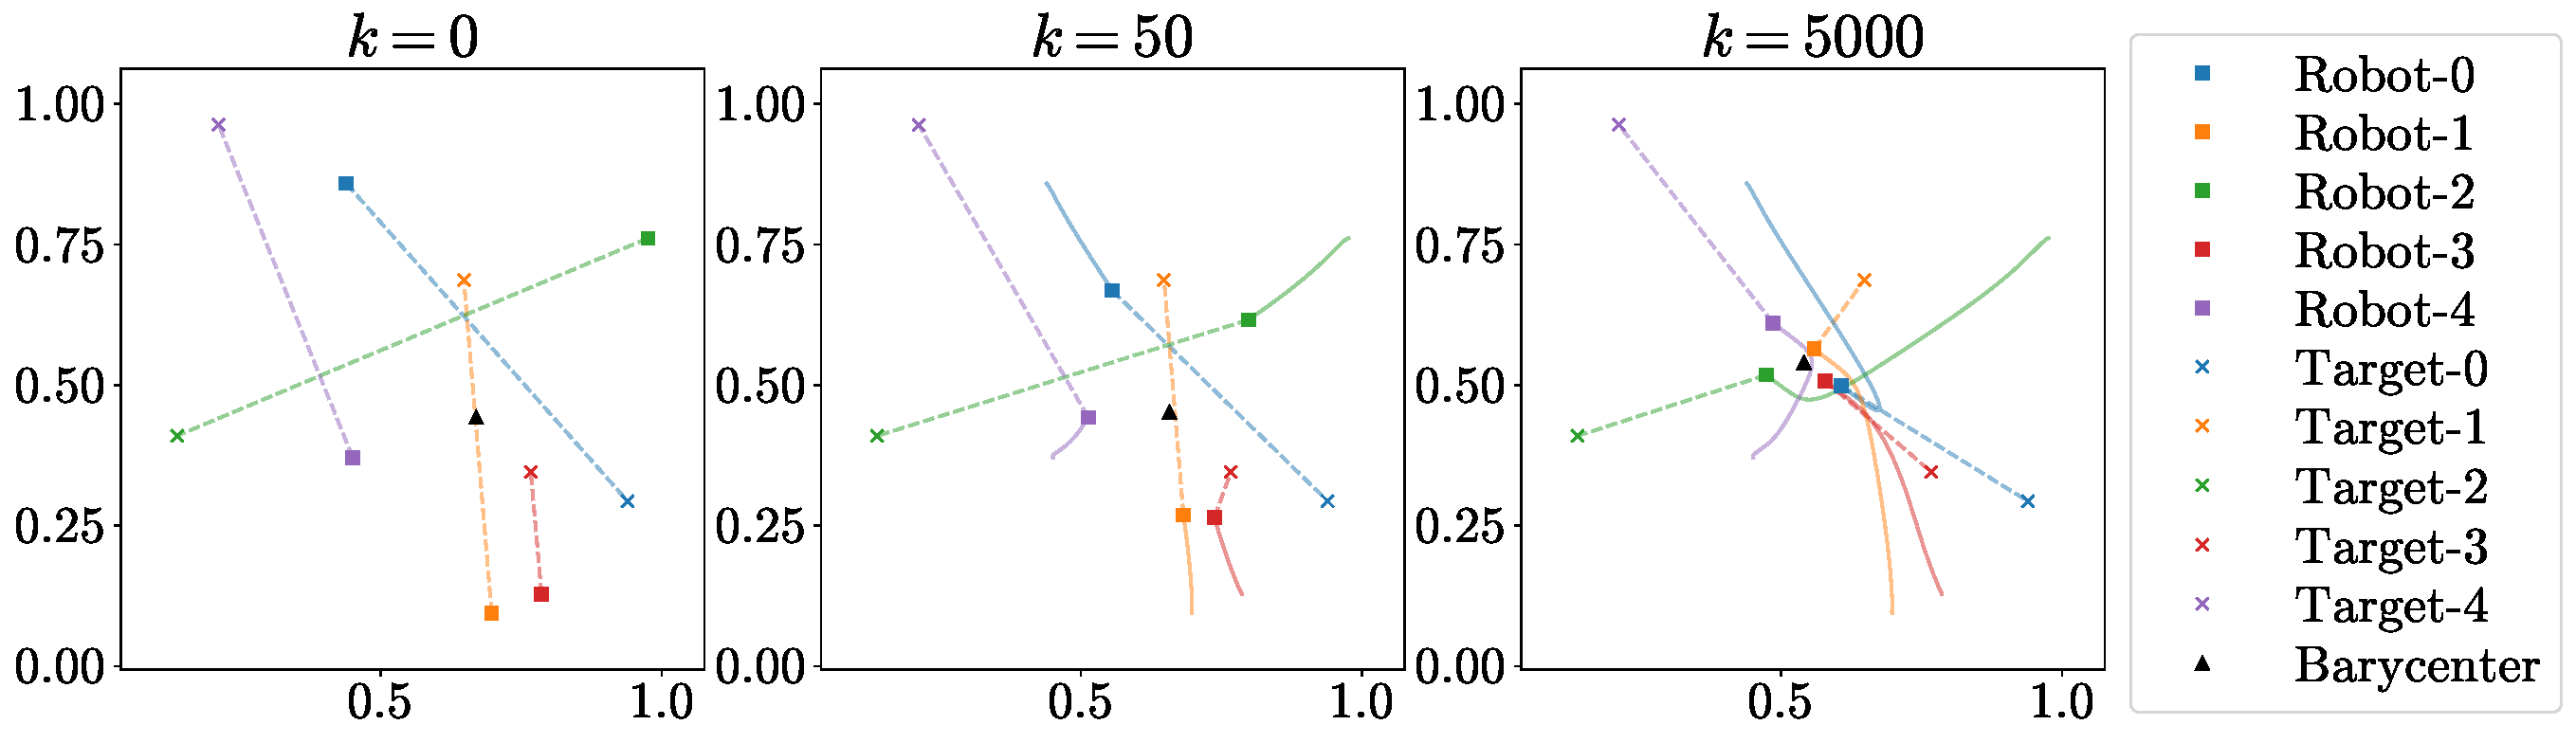
\includegraphics[width=0.9\linewidth]{./figs/aggregative/barycenter_anim/anim.pdf} 
      \caption{Frames with $5$ robots and loss that prioritizes the barycenter. Dashed lines connect robots to the targets and solid lines are the trajectories.}
      \label{fig:anim_barycenter}
\end{figure}

\begin{figure}[H]
      \centering
      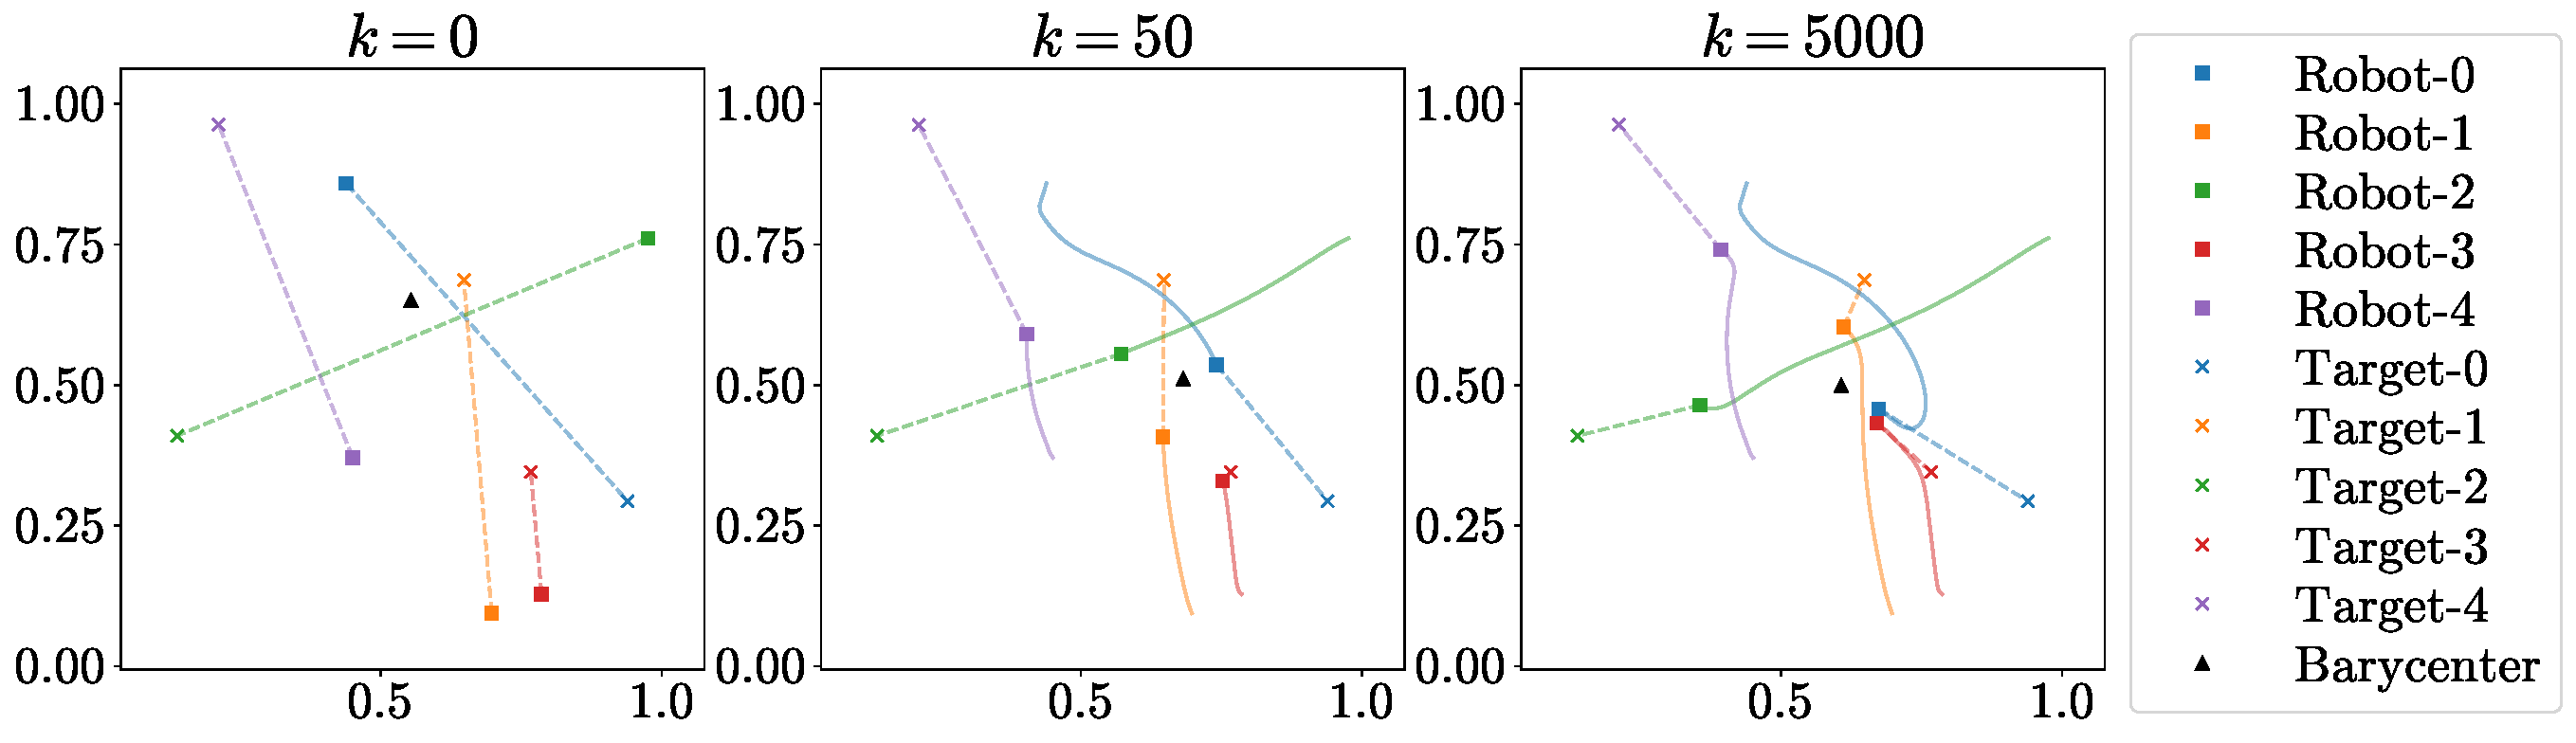
\includegraphics[width=0.9\linewidth]{./figs/aggregative/importance_anim/anim.pdf} 
      \caption{Frames with $5$ robots and barycenter that prioritizes robot $0$. Dashed lines connect robots to the targets and solid lines are the trajectories.}
      \label{fig:anim_importance}
\end{figure}




\chapter*{Conclusions}
\addcontentsline{toc}{chapter}{Conclusions} 

In this project, we tackled and experimented with the problems of multi-robot target localization and positioning. Regarding the multi-robot target localization problem, we tested the variation in performance under different graph patterns, number of agents, and dimensionality of the state variables. These tests showed that all graph patterns converge and higher graph connectivity helps in reaching it faster, which is more noticeable in case of larger numbers of agents. Other tests showed that under different noise distributions and intensities, tracking accuracy, as expected, is higher with more agents and worsens for stronger amounts of noise.

Regarding the multi-robot positioning problem, we first observed similar trends for all the configurations in terms of loss and gradient behavior, independently of the number of robots or the communication graph pattern. Additional experiments were performed and assessed visually by changing the loss hyperparameters affecting robots' importance, target vicinity, and fleet tightness. Results showed that the loss function provides flexibility in tuning these constraints and the robots' final positions were the expected ones.



% \bibliography{bibfile}{}


\end{document}